% interactapasample.tex
% v1.05 - August 2017

\documentclass[]{interact}

\usepackage{epstopdf}% To incorporate .eps illustrations using PDFLaTeX, etc.
\usepackage[caption=false]{subfig}% Support for small, `sub' figures and tables
%\usepackage[nolists,tablesfirst]{endfloat}% To `separate' figures https://it.overleaf.com/project/5bbc5c481ace70551dd2c703and tables from text if required
%\usepackahttps://it.overleaf.com/project/5bbc5c481ace70551dd2c703ge[doublespacing]{setspace}% To produce a `double spaced' document if required
%\setlength\parindent{24pt}% To increase paragraph indentation when line spacing is doubled
\usepackage{soul}
\usepackage{amsmath,amssymb} 
\usepackage[natbibapa,nodoi]{apacite}% Citation support using apacite.sty. Commands using natbib.sty MUST be deactivated first!
\setlength\bibhang{12pt}% To set the indentation in the list of references using apacite.sty. Commands using natbib.sty MUST be deactivated first!
\renewcommand\bibliographytypesize{\fontsize{10}{12}\selectfont}% To set the list of references in 10 point font using apacite.sty. Commands using natbib.sty MUST be deactivated first!
\theoremstyle{plain}% Theorem-like structures provided by amsthm.sty
\newtheorem{theorem}{Theorem}[section]
\newtheorem{lemma}[theorem]{Lemma}
\newtheorem{corollary}[theorem]{Corollary}
\newtheorem{proposition}[theorem]{Proposition}

\theoremstyle{definition}
\newtheorem{definition}[theorem]{Definition}
\newtheorem{example}[theorem]{Example}

\theoremstyle{remark}
\newtheorem{remark}{Remark}
\newtheorem{notation}{Notation}

\usepackage[pdftex,colorlinks=true,urlcolor=blue,citecolor=black,anchorcolor=black,linkcolor=black]{hyperref}
\usepackage{xcolor}
\newcommand{\mengyi}[1]{\textcolor{blue}{#1}}
\newcommand{\erica}[1]{\textcolor{red}{#1}}

\usepackage{algorithm} 
\usepackage{algorithmic} 
\renewcommand{\algorithmicrequire}{ \textbf{Input:}} %Use Input in the format of Algorithm
\usepackage{soul}
\usepackage{todonotes}

\begin{document}

%\articletype{ARTICLE TEMPLATE}% Specify the article type or omit as appropriate

\title{Generation of Mathematical Programming Representation From Discrete-Event Simulation Models}
\maketitle
\begin{abstract}

\end{abstract}

\section{Introduction}
Discrete Event Simulation (DES) is one of the most used tool for performance evaluation of %discrete event dynamic
complex systems and, hence, simulation--optimization algorithms are widely used %developed for optimizing the parameters of such systems. 
when performance evaluation has to be coupled with optimization, i.e., when the best system configuration, according to some criteria, has to be found meanwhile guaranteeing a given value of some performance measure.  
Most of the state--of--the--art simulation--optimization algorithms consider DES as a \textit{black--box} function, and the structure of DES models has been seldom studied. On the contrary, a minority of the simulation--optimization literature explores the structure of the DES models, and %that
such research is referred to as \textit{white--box} simulation--optimization. 
Under the black--box setting, simulation--optimization algorithms work in an iterative way, alternating simulation and optimization procedures, 
thus possibly leading to computational inefficiency if the number of iterations and/or the computation time per iteration increases pretty much. 
%and always require %huge amount of 
%many iterations to explore the %search 
%feasible region of the optimization problem, %and can be
%thus possibly leading to %computationally inefficient. 
%computational inefficiency.
The benefit of white--box simulation--optimization is the saving of simulation budget due to the fact that %since 
the optimization procedure is guided by the information contained in the structure of the DES model. However, the barrier to the use of white--box simulation--optimization is modeling DES as white--box, so that it eventually favors optimization. 

This work proposes a procedure to establish a white--box simulation model, which is an equivalent Mathematical Programming Representation (MPR) model, based on the well-known event--scheduling logic \citep{law2014simulation}. %for  
The procedure is applicable to certain types of DES models, and the assumptions that the DES model should satisfy is also presented in this work.
%Specifically, the modeling procedure, the assumptions which the DES model has to satisfy so that it can be applied and some examples are discussed. 

%In this work, we present how to establish an equivalent Mathematical Programming Representation (MPR) of Discrete Event Simulation (DES). The MPR depicts the dynamics of an event-scheduling approach of simulation modeling with a certain sample path. To develop the MPR, state variables, events, initial state, termination condition and the samples of the random variate should be provided. All requirement is also essential each time an event-scheduling algorithm is programmed. Furthermore, the proposed approach is quite routined. Thus, no extra knowledge or skills are required when one has the event-scheduling simulation implementation and wants to apply our approach. Besides the modeling approach, we provide the conditions to check before applying our approach, and discuss what the modifications can be done when some conditions are violated. Some examples are also given.

%Considering the literature on simulation--optimization, 
\cite{chan2008optimization} proposed a modeling framework to translate a DES model into an MPR model in a general sense. Their modeling framework is based on the Event Relationship Graph (ERG) of the system dynamics. To derive the MPR, % model, 
an ERG of the discrete event system has to be constructed and expanded to an elementary ERG (EERG) model, and a routine procedure can be applied to translate the EERG model into an MPR. %model. 
However, this procedure has some limitations. First, deriving an ERG is not an easy task, and the user has to pay quite much attention to detect all the event relationships and complete the triggering conditions between each pair of related events. %That 
The difficulty of developing ERG limits the wide spread of this procedure. 
Second, the modeling procedure is case--by--case depending on the event relationships, which means that the user has to analyze the event relationships one by one and identify which type of modeling, including the variables and constrains, he/she should apply for each event relationship. 
%which means the user has to first identify which situations he/she faces by analyzing the relationships between each couple of events in the EERG, and then choose the appropriate model, including the variables and constraints. 
This is quite %a burden
difficult, since EERG is an expansion of ERG; the resulting graph could be huge and writing down the complete MPR model could be even impossible.  

This work proposes a procedure that does not need % without plotting 
the ERG and %the modeling procedure 
can be used to automatically generate the MPR in a general--purpose programming language. Despite %taking different paths
being different, the MPRs proposed in this work and \cite{chan2008optimization} lead to %the 
equivalent results, which, in turn, are both equivalent to a simulation realization. Furthermore, the MPR of DES with event cancellation is another original contribution of this work. 

%When there is already a DES model, 
The benefit of developing an MPR might be not obvious (especially when there is already a DES model) due to the extremely high complexity of solving it. 
%One may be confused about the motivation of this work, i.e., why one wants the MPR when he/she has already a simulation model at hand, since the complexity of solving mathematical programming is usually high. 
In fact, we do not suggest to solve the MPR directly with state-of-the-art mathematical programming solvers. Instead, running the DES results in the optimal solution of MPR, and the MPR provides representation of the structure of the DES. With the vast theoretical and methodological results developed in the mathematical programming (MP) field, for instance sensitivity analysis as proposed by \cite{chan2008optimization}, the MPR of a simulation model favors the optimal design and control of the discrete event systems. 


Many works in the literature show the potentiality of this research direction. For instance, the gradient can be conveniently estimated from the simulation model, if the MPR is approximated into Linear Programming (LP) and %solving 
the dual can be conveniently obtained \citep{chan2008optimization, zhang2020simulation}. Moreover, if some of the parameters in the MPR are changed to decision variables, the MPR becomes an integrated simulation--optimization model. Solving the integrated model provides the optimal solution of the optimization problem \citep{matta2008simulation}. MP--based algorithms, such as linear programming approximation \citep{alfieri2012mathematical}, Benders decomposition \citep{weiss2015buffer}, column generation \citep{alfieri2020time}, have been applied to improve the efficiency of %solving the 
integrated MP model solution. 


The application of MPR--based simulation--optimization approaches is usually found in operations management of manufacturing and service systems. %The integrated simulation--optimization model has proved itself to be well suited in solving the buffer allocation problem \citep{zhang2020BAP}. %The most efficient approach to finding the sample--path global optimal of the buffer allocation problem of serial production line is developed based on it \citep{zhang2020BAP}. 
%Thanks to the flexibility of DES in evaluating complex systems, the buffer allocation problem of production systems with complex blocking mechanism, such as kanban control, base stock control, extended kanban control, can be managed \citep{pedrielli2015integrated}. Thanks to the flexibility of MPR in modeling optimization problems, problems involving real--valued decision variables such as optimal production rate \citep{tan2015mathematical}, bottleneck detection and throughput improvement problem \citep{zhang2020models} have all been well addressed and the sample--path global optimal solution can be obtained. %It is worthy to notice that, 
The flexibility of DES for complex system evaluation and of MPR for modeling optimization problems, allowed the integrated simulation-optimization approach to be effectively applied to buffer allocation problems \citep{zhang2020BAP}, even with complex blocking mechanisms \citep{pedrielli2015integrated} and to problems involving real values decision variables \citep{tan2015mathematical,zhang2020models}. 
Before the above mentioned works were proposed, there were many state--of--the--art heuristic approaches addressing those problems, but without any guarantee of global or local optimality. Thus, the development of MPR--based simulation--optimization has made its contribution in the research area of manufacturing and service system optimization.

%To extend the application of the MPR-based simulation optimization approaches, there is a need of modeling approach to translating DES into MPR under general settings.

The contribution of this work comes from various aspects. First, it proposes an MPR of DES from event-scheduling execution logic, which is the basement of many DES implementations. Thus, the procedure does not require much extra effort once one has an event-scheduling execution logic implemented. Second, it proposes the MPR of event cancellation, which is never studied in literature. Third, the vast literature in mathematical programming field can be applied to the resulting MPR, for instance, gradient estimation. Last, the proposed MPR can be easily transformed into an MPR of optimization over design parameters of the DES, which are common optimization problems in operations management field.  


The rest of the paper is organized as follows. Section \ref{sec:MPR} describes generation of the MPR of a DES model, including a brief introduction of event-scheduling algorithm, the assumptions for applying the propose procedure, to the modeling steps requiring users manually work, and the MPR itself generated automatically based on the model. Section \ref{sec:app} shows several examples of DES and the generated MPR, whose equivalence has been validated. Section \ref{sec:discussion} closes this work with a discussion. 

\section{MPR generation procedure} \label{sec:MPR}
\subsection{Event-scheduling execution logic of DES } \label{sec:SimAlgo}

The event-scheduling approach is the logic behind all the major DES software and used by practitioners when developing simulation codes with general purpose languages \citep{law2014simulation}. For sake of completeness, we briefly describe the logic as shown in Figure \ref{Fig:SimAlgo}. The fundamental elements are the system state and the events. The system state is a collection of state variables to describe the system at a particular time, while an event is everything whose execution can change the system state. %An event execution can lead to the change of system state.%, the events of the same type change the system state with the same function
All the already scheduled but not yet executed events are stored in the future event list together with their occurring times. %The event list contains the scheduled but not executed events together with occurring times. 
When simulation is launched, the system state and the future event list is initialized with user-defined values, and the simulation clock is set to zero. The event with the earliest occurring time in the future event list will be executed, and the system evolves into a new state together with the simulation clock. The new state may enable to schedule new events, i.e., adding new event together with execution time to the future event list, or cancel events, i.e., removing some event executions from the future event list. There is usually a delay between the time when an event is added to the event list and the time when the event is executed. %, but the delay might be equal to zero or positive. 
In the following, we refer the time when an event is added to the event list as the \textit{scheduling time}, and the time when an event is executed as the \textit{execution time}. The algorithm will terminate when some given condition is met or when a given value for the simulation clock is reached.

\begin{figure}[h]
	\centering
	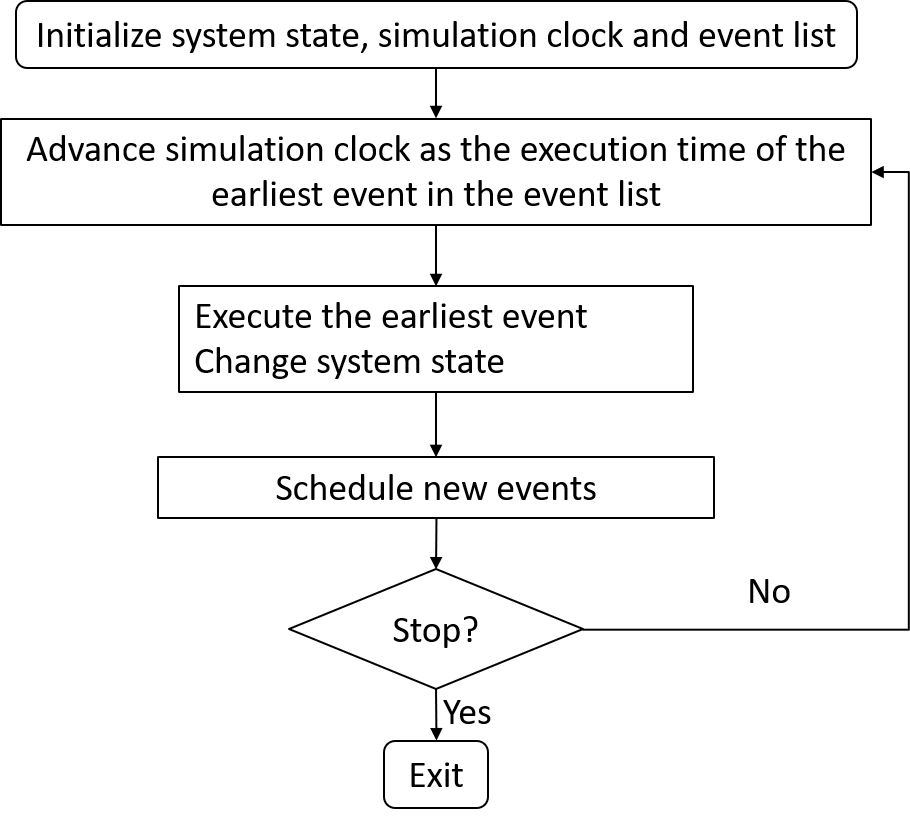
\includegraphics[width=0.6\textwidth]{Figures/EventSimAlgo.png}
	\caption{Event-scheduling simulation algorithm.}
	\label{Fig:SimAlgo}
\end{figure}

%\section{Mathematical programming representation of DES}
In the following of this section, a procedure to translate DES models into MRP models, based on the event-scheduling approach, is introduced. Before presenting the procedure, the assumptions that the DES model has to satisfy in order to have the procedure applicable, are described.

\subsection{Assumptions}

To apply the procedure proposed in this work, the following assumptions must be satisfied.


\begin{enumerate}
	\item State variables are integer.
	\item For all the events $e^{\xi}$ of type $\xi$, the \textit{scheduling conditions} and the \textit{cancellation conditions} are in the form $a^{\xi}_s\le s \le c^{\xi}_s$ for certain state variable $s$. When multiple state variables are involved, they are combined using the logical operator ``AND".
	%and combined with logic operator ``AND" when multiple state variables are involved, where $a^{\xi,s}$ and $b^{\xi,s}$ are given.
	%\item The scheduling condition of an event is independent of the history and not changed along time.% (It could be possible to define more state variables in case of history dependence and time-variant scheduling conditions.)
	%\item An event execution of $e^{\xi}$ leads to (integer) increment or decrement equal to $\Delta^{\xi}_s$ of certain state variables $s$, and $\Delta^{\xi}_s$ is not changed along time. (A direct evaluation can be modeled in this way.)
	\item The delay between the scheduling time and the execution time of event $e^{\xi}$ are independent and identically distributed random variables. %(\textit{This point is different from ERG. In ERG, the delay is dependent on the edge, i.e, a couple of events, but I consider delay dependent on a single event.})
	\item When more than one event in the event list have the same execution time% as the earliest execution time
	, the execution sequence is immaterial, i.e., each execution sequence leads to the same new system state and the same new event list when the simulation clock is advanced.	
	%	the system state, the event list and the number of past executions of each event type are independent of the sequence of execution when the simulation clock is advanced.
	\item Simulation terminates when the total number of event executions reaches a known value $K$.
	%Simulation terminates when the number of execution of each event $e^{\xi}$ reaches $N^{\xi}$, which is known, i.e., the number of entities in the system is known. 
	%\item Only event with positive-delay between scheduling and execution can be canceled.
\end{enumerate}

The first assumption requires the state variables to be integer. Integer variables widely exist in DES models, such as number of jobs in buffers, idle servers, and binary variables to model system behavior and control. A discrete state variable can be translated into an integer variable or a set of binary variables. For real-valued state variables, it can be approximately discretized. Thus, the first assumption is fairly general.

The second assumption is, instead, more strict. However, if a model does not satisfy this condition, one can consider to introduce extra binary variables to satisfy assumption (2). For instance, if the condition to schedule event $e^{\xi}$ is $s\le a^{\xi}_s \ OR\ s\ge b^{\xi}_s$, a binary variable $s^{'}$ can introduced to the model, and $s^{'}$ is equal to one if and only if 
$s\le a^{\xi}_s \ OR\ s\ge b^{\xi}_s$. Thus, at the cost of increase of model complexity, violation of assumption (2) can be overcome.

As for the third assumption, the delay represents usually service or inter-arrival time. For example, if an event represents the finishing of a job on a machine, it is scheduled (i.e., put in the list) when the job starts its processing, and it will be executed when the jobs will be finished, i.e., the time between scheduling and execution is the job processing time. 
If the condition is not met, i.e., if the delay is not an iid random variate, it can be splitted into several events so that each event has iid delay. For instance, if the distribution of service time depends on the job type, the event of \textit{finishing} a job should be splitted such that the \textit{finishing} of each job type is represented by one event. 
 
The fourth assumption, in practice, says that the execution time is the only attribute of priority for the event executions in the future event list. If one would like to specify a different priority of some events having the same execution time, he/she can specify the priority by adding the event with lower priority to the event list after the execution of the event with higher priority, which can be done by introducing extra binary variables. This assumption also implies that only events with positive delay can be events with cancellation. Let us assume that there is a zero-delay event $e^{\xi}$ with cancellation. After an execution of $e^{\xi}$ is added to the future event list, it can be executed immediately, since it is zero-delay. Otherwise, if there is a certain time before executing it, the cancellation condition of $e^{\xi}$ is true, the execution will be canceled, and assumption (4) is violated. Thus,  only event with positive-delay can be canceled.

The fifth condition specifies termination condition of the event-scheduling algorithm. %Specifically, for queueing systems, the termination condition usually refers to the number of jobs passing through each station.


%The proposed procedure cannot handling event cancellation, as stated in the last assumption.

\subsection{Mathematical programming generation procedure} \label{sec:MPR_procedure}

To implement the event-schedule algorithm and generate MPR, events and state variables should be first defined. For instance, to simulate a G/G/m system, three events and two state variables are essential. The three events represent job arrival, service start and service finish, and are denoted by $e^{arr}$, $e^{ss}$ and $e^{sf}$, respectively. The two state variables represent the number of jobs in the queue and the number of occupied servers, and are denoted by $q$ and $g$, respectively. State variable $q$ is non-negative integer, and $g$ can be any integer between $0$ and $m$, which is number of servers. 

For each event $e^{\xi}$, the condition to schedule, the condition to cancel, the distribution of delay between scheduling and execution $T^{\xi}$, maximal number of executions in the future event list $\beta^{\xi}$ and the state variable changes upon execution are also necessary. The condition to schedule, the condition to cancel, the distribution of delay between scheduling and execution $T^{\xi}$ should satisfy the assumption (2) and (3). In the future event list, there is usually an upper bound of number of executions of the each event $e^{\xi}$, represented by $\beta^{\xi}$. For instance, to simulate an arrival process, the maximal number of arrival in the event list is equal to $1$, since only after a previous arrival, a new arrival can be scheduled with a delay equal to the inter-arrival time. For events with $\beta^{\xi}$ equal to one, we name it as \textit{single-execution} events, and we name events with $\beta^{\xi}$ greater than one as \textit{multi-execution} events. All the zero-delay events are defined as single-execution, because when the delay between scheduling and execution of an event is zero, multiple executions are equivalent to sequential scheduling of a single-execution event. For positive-delay events $e^{\xi}$, we introduce the following procedure. A \textit{counting} event ${e}^{\tilde{\xi}}$ and counting variable $u^{\xi}$ are created artificially. The counting event ${e}^{\tilde{\xi}}$ is zero-delay, with the same scheduling condition as $e^{\xi}$. %Each time the condition to schedule is true, an execution of ${e}^{\tilde{\xi}}$ is added to the future event list. 
When ${e}^{\tilde{\xi}}$ is actually executed, an execution of $e^{\xi}$ is added to the future event list. Then, if the condition to schedule event $e^{\xi}$ is still true, another ${e}^{\tilde{\xi}}$ is scheduled, therefore, simultaneous scheduling of multiple executions of event $e^{\xi}$ can be done in a sequential way without advancing simulation clock. The counting variable $u^{\xi}$ represents the number of executions of $e^{\xi}$ in the future event list, and its value is incremented by one when counting event $e^{\tilde{\xi}}$ is executed and decremented by one when event $e^{\xi}$ is executed. If event $e^{\xi}$ is canceled, $u^{\xi}$ is reset to zero. Since the maximal number of executions of $e^{\xi}$ is equal to $\beta^{\xi}$, the inequality $u^{\xi}\le\beta^{\xi}-1$ should be included into condition to schedule it, as well as event $e^{\tilde{\xi}}$. Besides integer $K$, which represents the total number of executions before simulation termination, the number of executions of each event $\xi$ should also be provided, denoted by $N^{\xi}$. It is not necessary that $N^{\xi}$ is exactly equal to the number of executions of event $\xi$ in the simulation run, instead, it could be an upper bound of it. Generally speaking, $N^{\xi}$ can be equal to K, but the smaller the value, the fewer number of variables are in the MPR, thus a simpler model will be developed consequently.

Table \ref{tab:ggm_1} shows the example of G/G/m. Since event cancellation is not relevant, condition to cancel is not showed. Event $e^{arr}$ is a positive-delay event, as explained above. %and one execution can be scheduled as soon as the previous job arrives with a delay equal to a sample from inter-arrival time distribution $T^{arr}$. 
A counting event of $e^{arr}$, i.e., $e^{\tilde{arr}}$, and a counting variable $u^{arr}$ is defined. The condition to schedule $e^{arr}$ is that $u^{arr}$ is equal to zero. When $e^{arr}$ is executed, one job arrives to the system, and queue level $q$ is increased by one. Event $e^{ss}$ is a zero-delay event, thus, single-execution. The condition to schedule $e^{ss}$ is that there is one job waiting in the queue and one server available. Upon execution of $e^{ss}$, queue level is reduced by one, and number of occupied server in increase by one. Event $e^{fs}$ is a multiple-execution positive-delay event, it is scheduled immediately after $e^{ss}$ is executed, and the delay until its execution is equal to the service time, i.e., a sample from $T^{sf}$. Therefore, event $e^{ss}$ can be regarded as the counting event of $e^{sf}$. Furthermore, state variable $g$ is the counting variable of $e^{sf}$. %If the simulation terminates with $N$ jobs processed by the system, the total number of executions of all events is equal to $N$.

\begin{table}[h]
	\begin{tabular}{lllllll}
		\multicolumn{7}{l}{\textbf{Zero-delay events}}\\ \hline
		Variable&Event &  \multicolumn{4}{c}{Condition to schedule} & State change\\\hline%&$N^{\xi}$
		$e^{\tilde{arr}}$ & Counting arrival&  \multicolumn{4}{c}{$u^{arr}\le0$} & $u^{arr}${\footnotesize++} \\
		$e^{ss}$& Start 	& \multicolumn{4}{c}{$1\le q, g\le m-1$} & $g${\footnotesize++},$q${\small-}{\small-}  \\
		\multicolumn{7}{l}{\textbf{Positive-delay events}}\\ \hline
		Variable&Event & Delay& $e^{\tilde{\xi}}$& $u^{\xi}$ &$\beta^{\xi}$& State change\\\hline
		$e^{arr}$& Arrival & $T^{arr}$& $e^{\tilde{arr}}$& $u^{arr}$ &1& $q${\footnotesize++},$u^{arr}${\small-}{\small-} \\	
		$e^{sf}$& Finish & $T^{sf}$& $e^{ss}$& $g$  &m& $g${\small-}{\small-} \\\hline
	\end{tabular}
	\caption{Events to simulate G/G/m system.}
	\label{tab:ggm_1}
\end{table}


\subsection{Mathematical programming model}


The MPR represents the dynamics of the simulated system,  equivalent to the event-scheduling algorithm. Specifically, event scheduling time, event execution time and state variable changes during simulation can all be seen in the MPR as decision variables. The $i$-th scheduling time and its execution time of event $e^{\xi}$ are denoted by $e^{\xi,0}_{i}$ and $e^{\xi,1}_{i}$, respectively. The system state changes with event executions, and we organize the executions into a single series and use $\mathcal{E}_k$ to denote the $k$-th execution time, i.e., the simulation clock values when an event is executed. The index $i$ represents the sequence of scheduling or execution of a specific event type, and the index $k$ represents the sequence of execution of general event types in the following of this work. $e^{\xi,0}_{i}$, $e^{\xi,1}_{i}$ and $\mathcal{E}_k$ are all real-valued and non-negative. The variables $u^s_k$ is used to denote the value of state variable $s$ just after the $k$-th execution, i.e., just after $\mathcal{E}_k$ and before scheduling or canceling any event. The variables $u^s_k$ are integer according to assumption (1). The initial system state is given as $u^s_0$. Some binary variables are also used in the MPR, and they will be introduced in the following, during the explanation of the model. 

The set of all event types $\xi$ is denoted by $\mathbb{X}$. $\mathbb{I}^{\xi}$ denotes the set $\{1,...,N^{\xi}\}$, which is the number of executions of event $e^{\xi}$, and $\mathbb{K}$ denotes the set $\{1,...,K\}$, which is the total number of event executions. $\mathbb{S}$ denotes the set of all state variables. $\mathbb{S}^{\xi}$ and $\mathbb{S}^{\bar{\xi}}$ denote the set of state variables relevant to scheduling and cancellation conditions of event $e^{\xi}$, respectively.

\subsubsection{Event execution time} \label{sec:const_A}
The first group of mathematical relationships, denoted by group A, are the constraints binding executions $e^{\xi,1}_i$ and $\mathcal{E}_k$. Binary variables $w^{\xi}_{i,k}$ are used, and $e^{\xi,1}_i$ and $\mathcal{E}_k$ are binded if and only if $w^{\xi}_{i,k}$ is equal to one, i.e., the $k$-th event execution is the $i$-th execution of event $e^{\xi}$, as shown in constraints (A1) and (A2). Constraints (A3) and (A4) state that each $e^{\xi,1}_i$ can be binded to at most one $\mathcal{E}_k$, while each $\mathcal{E}_k$ must binded to one and only one $e^{\xi,1}_i$. Constraints (A5) imply that the $\mathcal{E}_{k}$ are temporally sequenced with index $k$, i.e., the $k$-th execution cannot be later than the $(k-1)$-th execution. Constraint (A6) implies that the simulation clock is initialized to zero. Constraints (A7) implies that the scheduled event is executed after a time delay equal to the sample from the random distribution $T^{\xi}$.
%the index executions of the same event type is sequenced along with the index of $\mathcal{E}_k$.

\begin{eqnarray}
e^{\xi,1}_i-\mathcal{E}_k\ge M(w^{\xi}_{i,k}-1) & \forall\ \xi\in\mathbb{X},i\in \mathbb{I}^{\xi},k\in \mathbb{K}&(A1)\nonumber\\
\mathcal{E}_k-e^{\xi,1}_i\ge M(w^{\xi}_{i,k}-1) & \forall\ \xi\in\mathbb{X},i\in \mathbb{I}^{\xi},k\in \mathbb{K}&(A2)\nonumber\\
\sum_{k\in \mathbb{K}} w^{\xi}_{i,k} \le 1& \forall\ \xi\in\mathbb{X},i\in \mathbb{I}^{\xi}&(A3)\nonumber\\
\sum_{\xi\in \mathbb{X}}\sum_{i\in \mathbb{I}^{\xi}} w^{\xi}_{i,k} =1&\forall\ k\in \mathbb{K}&(A4)\nonumber\\
\mathcal{E}_{k}-\mathcal{E}_{k-1}\ge 0&\forall\ k\in \mathbb{K}&(A5)\nonumber\\
%\sum_{k\in \mathbb{K}} kw^{\xi}_{i,k} - \sum_{k\in \mathbb{K}} kw^{\xi}_{i-1,k} \ge 1&  \forall\ \xi\in\mathbb{X},i\in \mathbb{I}^{\xi}&(A6)\nonumber\\
\mathcal{E}_0 = 0&&(A6)\nonumber\\
e^{\xi,1}_{i} - e^{\xi,0}_{i} = t^{\xi}_{i} & \forall \xi\in\mathbb{X}, i\in \mathbb{I}^{\xi}&(A7) \nonumber
\end{eqnarray}

%\subsubsection{Multiple-execution events}\label{sec:const_B}
%The second group of constraints, denoted by group B, are the constraints binding event scheduling $e^{\xi,0}_i$ and event execution $e^{\xi,1}_{i^{'}}$, and the time delay between which is a sample of $T^{\xi}$. If the event is single--execution, i.e., the maximum number of executions in the event list is equal to one, the $i$-th execution $e^{\xi,1}_i$ is the $i$-th scheduled one, as in constraints (B1), where $t^{\xi}_{i}$ is a sample of $T^{\xi}$. Thus, the variable $e^{\xi,1}_{i} $ can be replaced by $e^{\xi,0}_{i} + t^{\xi}_{i}$ and the MPR model can reduced.
%\begin{eqnarray}
%e^{\xi,1}_{i} - e^{\xi,0}_{i} = t^{\xi}_{i} & \forall \xi\in\mathbb{X}, i\in \mathbb{I}^{\xi}&(B1) \nonumber
%\end{eqnarray}

%If event $e^{\xi}$ is a multi-execution event, a late scheduled execution can overtake an early scheduled one, since the delay time between scheduling and execution is a random variate. For instance, in a G/G/2 queue, the departure of the first job is the first scheduled departure event, but it may be not the first to execute, if its service time is pretty long so that the second starting job leaves the system earlier. Thus, binary variables $y^{\xi}_{i,i^{'}}$ are introduced, and the $i^{'}$-th execution of event $e^{\xi}$ is the $i$-th scheduled one with a delay equal to $ t^{\xi}_{i}$, a sample of $T^{\xi}$, when $y^{\xi}_{i,i^{'}}$ is equal to one, as in constraints (B2) and (B3). Constraints (B4) and (B5) show that each execution can be binded to one and only one scheduling. Constraints (B6) imply that the $i$-th scheduling cannot be binded to an execution earlier than the $(i+\beta^{\xi})$-th, since at most $\beta^{\xi}$ executions are allowed to be in the list at the same time. For the same reason, constraints (B7) state that $i^{'}$-th execution cannot be binded to the scheduling later than the $(i^{'}-\beta^{\xi})$-th. For instance, in a G/G/2 queue, the third arrival job cannot be the first departure job, since its service starts after the first departure.


\subsubsection{Constraints for scheduling new events}\label{sec:const_C}
The second group of constraints, denoted by group B, state that an execution of event $e^{\xi}$ can be scheduled right after $\mathcal{E}_k$ if the condition for scheduling an event $e^{\xi}$ is true. Binary variables $x^{\xi}_{i,k}$ are used, and $x^{\xi}_{i,k}$ equal to one represents that the $i$-th scheduling of event $e^{\xi}$ is enabled right after $\mathcal{E}_k$, as in constraints (B1) and (B2). 

For zero-delay events, constraints (B3) to (B12) are relevant. Binary variables $z^{\xi}_{k}$ are introduced, and $z^{\xi}_{k}$ equal to one represents that it is obligatory to schedule an event $e^{\xi}$ right after execution $\mathcal{E}^k$. If and only if the state variables satisfy the condition to schedule, and all the previously scheduled executions are executed, a new execution of event $e^{\xi}$ can be scheduled. Constraints (B3) and (B4) imply that if $z^{\xi}_k$ is equal to one, the state variables satisfy the condition to schedule. Moreover, a set of binary variables $v^{\xi,s,0}_k$ and $v^{\xi,s,1}_k$ are used to verify if the condition to schedule is false. Specifically, constraints (B5) state that if  $v^{\xi,s,0}_k$ is equal to one, $u^s_k$ will be smaller than $a^{\xi,s}$, and hence, the inequality $a^{\xi}_s\le s$ is violated. Similar for constraints (B6), if $v^{\xi,s,1}_k$ is equal to one, $s \le c^{\xi}_s$ is violated. %Constraints (C8) imply that if $z^{\xi}_k$ is equal to one, then all the previously scheduled execution of event $e^{\xi}$ have been executed. 
Binary variable $v^{\xi,\beta}_k$ equal to one represents that  there is a schedule execution not being executed yet, as constraints (B7). $v^{\xi,\beta}_{0}$ is initialized by zero, since the future event list is empty when the algorithm is initialized. Based on $v^{\xi,\beta}_{k-1}$, $v^{\xi,\beta}$ is increased by one if $e^{\xi}$ is scheduled after $\mathcal{E}_{k-1}$ and decreased by one if $e^{\xi}$ is executed as $\mathcal{E}_{k}$. 
Constraints (B8) specify that $z^{\xi}_k$ equal to zero only if at least one of the above mentioned conditions is violated, i.e., either the condition to schedule is violated, or there is already an execution in the future event list. Constraints (B9) show that if $z^{\xi}_k$ is equal to one, one execution of $e^{\xi}$ is scheduled right after execution $\mathcal{E}_k$. Constraints (B10) state that all executions of $e^{\xi}$, indexed from 1 to $N^{\xi}$, are scheduled for at most once. Constraints (B11) depict that if the $(i+1)$-th execution is scheduled before simulation termination, it must be scheduled after the $i$-th execution is executed. Constraints (B12) states that an execution cannot be executed before being scheduled, if it is executed before simulation termination. 

For positive-delay events, constraints (B13) are relevant. (B13) show that one execution of positive-delay event $e^{\xi}$ is scheduled after each execution of its counting event $e^{\tilde{\xi}}$.

For all events, constraints (B14) to (B16) are relevant. Constraints (B14) show that before simulation termination, if the $i$-th execution of event $\xi$ is not scheduled, then $(i+1)$-th execution will not be scheduled. Constraints (B15) state that before simulation termination, if the $i$-th execution of event $\xi$ is not scheduled, then it will not be executed. Constraints (B16) depict that the $(i+1)$-th execution of event $\xi$ must be scheduled after the $i$-th execution.


\begin{eqnarray}
e^{\xi,0}_i-\mathcal{E}_{k} \ge M(x^{\xi}_{i,k}-1)& \forall\ \xi\in \mathbb{X},k\in \mathbb{K},i\in \mathbb{I}^{\xi}&(B1)\nonumber\\
\mathcal{E}_{k} -e^{\xi,0}_i\ge M(x^{\xi}_{i,k}-1)&\forall\ \xi\in \mathbb{X},k\in \mathbb{K},i\in \mathbb{I}^{\xi}&(B2)\nonumber\\
u^s_k - a^{\xi,s} \ge M(z^{\xi}_{k}-1)&\forall\ \xi\in \mathbb{X},k\in \mathbb{K},s\in \mathbb{S^{\xi}},\ t^{\xi} = 0&(B3)\nonumber\\
c^{\xi,s} - u^s_k \ge M(z^{\xi}_{k}-1)&\forall\ \xi\in \mathbb{X},k\in \mathbb{K},s\in \mathbb{S^{\xi}},\ t^{\xi} = 0&(B4)\nonumber\\
( a^{\xi,s}-1) - u^s_k \ge M(v^{\xi,s,0}_k-1) & \forall\ \xi\in \mathbb{X},k\in \mathbb{K},s\in \mathbb{S^{\xi}},\ t^{\xi} = 0 &(B5)\nonumber\\
u^s_k -  (c^{\xi,s}+1) \ge M(v^{\xi,s,1}_k-1) & \forall\ \xi\in \mathbb{X},k\in \mathbb{K},s\in \mathbb{S^{\xi}},\ t^{\xi} = 0 &(B6)\nonumber\\
%\sum_{k^{'}=1}^{k}\sum_{i\in \mathbb{I}^{\xi}} w^{\xi}_{i,k^{'}} - \sum_{k^{'}=0}^{k-1}\sum_{i\in \mathbb{I}^{\xi}} x^{\xi}_{i,k^{'}} \ge z^{\xi}_{k}-1&\forall\ \xi\in \mathbb{X},k\in \mathbb{K},s\in \mathbb{S},\ t^{\xi} = 0&(C8)\nonumber\\
v^{\xi,\beta}_k = v^{\xi,\beta}_{k-1} - \sum_{i\in \mathbb{I}^{\xi}}w^{\xi}_{i,k} + z^{\xi}_{k-1} & \forall\ \xi\in \mathbb{X},k\in \mathbb{K},\ t^{\xi} = 0 &(B7)\nonumber\\
%\sum_{k^{'}=0}^{k-1}\sum_{i\in \mathbb{I}^{\xi}} x^{\xi}_{i,k^{'}}- \sum_{k^{'}=1}^{k}\sum_{i\in \mathbb{I}^{\xi}} w^{\xi}_{i,k^{'}} \ge v^{\xi,\beta}_k & \forall\ \xi\in \mathbb{X},k\in \mathbb{K},\ t^{\xi} = 0 &(C8)\nonumber\\
%\sum_{k\in\mathbb{K}} z^{\xi}_{k} = N^{\xi}&\forall\ \xi\in \mathbb{X},s\in \mathbb{S},\ t^{\xi} = 0&(C7)\nonumber\\
%\sum_{k^{'}=0}^{k-1} z^{\xi}_{k^{'}} \ge N^{\xi}v^{\xi,N}_k & \forall\ \xi\in \mathbb{X},k\in \mathbb{K},\ t^{\xi} = 0 &(B8)\nonumber\\
1 - z^{\xi}_{k} \le \sum_{s\in \mathbb{S}^{\xi}} v^{\xi,s,0}_k + \sum_{s\in \mathbb{S}^{\xi}} v^{\xi,s,1}_k+v^{\xi,\beta}_k&\forall\ \xi\in \mathbb{X},k\in \mathbb{K},\ t^{\xi} = 0&(B8)\nonumber\\
\sum_{i\in \mathbb{I}^{\xi}} x^{\xi}_{i,k} = z^{\xi}_k&\forall\ \xi\in \mathbb{X},k\in \mathbb{K},\ t^{\xi} = 0&(B9)\nonumber\\
\sum_{k\in \mathbb{K}} x^{\xi}_{i,k} \le 1& \forall\ \xi\in \mathbb{X},i\in \mathbb{I}^{\xi},\ t^{\xi} = 0&(B10)\nonumber\\
\sum_{k\in \mathbb{K}} kx^{\xi}_{i+1,k} - \sum_{k\in \mathbb{K}} kw^{\xi}_{i,k} \ge M(\sum_{k\in \mathbb{K}} x^{\xi}_{i+1,k}-1)&  \forall\ \xi\in \mathbb{X},i\in \mathbb{I}^{\xi}, t^{\xi} = 0&(B11)\nonumber\\
\sum_{k\in \mathbb{K}} kw^{\xi}_{i,k} - \sum_{k\in \mathbb{K}} kx^{\xi}_{i,k} \ge 1 +M(\sum_{k\in \mathbb{K}} w^{\xi}_{i,k}-1) &\forall\ \xi\in \mathbb{X}, i\in \mathbb{I}^{\xi}, t^{\xi} = 0&(B12) \nonumber\\
x^{\xi}_{i,k} = w^{\tilde{\xi}}_{i,k}&  \forall\ \xi\in \mathbb{X},i\in \mathbb{I}^{\xi}, t^{\xi} > 0&(B13)\nonumber\\
\sum_{k\in \mathbb{K}} x^{\xi}_{i+1,k} - \sum_{k\in \mathbb{K}} x^{\xi}_{i,k} \le 0&  \forall\ \xi\in \mathbb{X},i\in \mathbb{I}^{\xi}&(B14)\nonumber
\end{eqnarray}
\begin{eqnarray}
\sum_{k\in \mathbb{K}} w^{\xi}_{i,k}-\sum_{k\in \mathbb{K}} x^{\xi}_{i,k} \le 0&  \forall\ \xi\in \mathbb{X},i\in \mathbb{I}^{\xi}&(B15)\nonumber\\
\sum_{k\in \mathbb{K}} kx^{\xi}_{i+1,k} - \sum_{k\in \mathbb{K}} kx^{\xi}_{i,k} \ge 1+M(\sum_{k\in \mathbb{K}} x^{\xi}_{i+1,k}-1)&  \forall\ \xi\in \mathbb{X},i\in \mathbb{I}^{\xi}&(B16)\nonumber
\end{eqnarray}


%First, multiple execution events should all have positive delay. In fact, when the delay between scheduling and execution of an event is zero, multiple executions is equivalent to sequential scheduling of a single-execution event. For the event $e^{\xi}$ with strictly positive delay, the following routine should be followed to formulate a correct MPR. An event ${e}^{\tilde{\xi}}$ that has the same scheduling condition as $e^{\xi}$ and is zero-delay should be included artificially. The reason to introducing $e^{\tilde{\xi}}$ is not to limit the number of executions, but to allow scheduling of multiple executions, instead, thus ${e}^{\tilde{\xi}}$ is named as the \textit{duplicating} event of event $e^{\xi}$. According to constraints (C9), at most one execution can be scheduled after execution of $\mathcal{E}_{k}$. To schedule multiple executions, the artificial event is used to make sure that the number of executions of event $e^{\xi}$ can reach $\beta^{\xi}$ if the condition to schedule is satisfied. Each time the condition to schedule $e^{\xi}$ is true, event ${e}^{\tilde{\xi}}$ can also be scheduled. Thus, the $i$-th scheduling of event $e^{\xi}$ and ${e}^{\tilde{\xi}}$ should be enabled by the same execution, as stated in constraints (C11), and there is no need to repeat constraints (C3) to (C9) for event ${e}^{\tilde{\xi}}$. In many cases, an event can play the role of duplicating event for another event, so there is no need to create a duplicating event. For instance, a DES model of G/G/m queue is composed of three events, which are arrival, start and finish. The condition to schedule both start and finish events is an idle server and a job in the queue, and start event is zero-delay, and finish event is positive-delay. Thus, the start event can be used as the duplicating event for finish event

\subsubsection{Constraints for event cancellation}\label{sec:const_D}
The third group of constraints, denoted by group C, state that executions of event $e^{\xi}$ in the event list are canceled right after $\mathcal{E}^k$ if the cancellation condition is true. Similar to constraints (B3) to (B6), constraint (C1) to (C4) show that if binary variables $z^{\bar{\xi}}_{k}$ are equal to one, then the cancellation condition of $e^{\xi}$ is true right after $\mathcal{E}^k$, where binary variable $z^{\bar{\xi}}_{k}$, $v^{\bar{\xi},s,0}_k$ and $v^{\bar{\xi},s,1}_k$ are the counter part of $z^{\xi}_{k}$, $v^{\xi,s,0}_k$ and $v^{\xi,s,1}_k$, but for event cancellation rather than event scheduling. %Constraints (D5) and (D6) show that if $z^{\bar{\xi}}_{k}$ is equal to one, there is at least one execution of event $e^{\xi}$ in the future event list, and that if $v^{\bar{\xi},\beta}_k$ equal to one, there is no execution. 
Constraints (C5) show that $z^{\bar{\xi}}_{k}$ can be equal to zero, only if the cancellation condition is false. 

%An execution is canceled if there is a moment after its scheduling and before its execution such that the cancellation condition is true, i.e., there is certain $k$ such that $z^{\bar{\xi}}_{k}$ is equal to one. 
The $i$-th execution of event $e^{\xi}$ is canceled after execution $\mathcal{E}_k$ if the cancellation condition is true for a certain $k$ after its scheduling and before its execution. In the MPR, any scheduled executions are executed, no matter if it is canceled. However, the canceled executions will not lead to any state change. For the $i$-th execution of event $e^{\xi}$, integer variables $k^{\xi,0}_i$ represent the index of execution that scheduled it and $k^{\xi,1}_i$ represent its execution sequence. The value of $k^{\xi,0}_i$ and $k^{\xi,1}_i$ is calculated as constraints (C6) and (C7). Thus, the $i$-th execution of event $e^{\xi}$ will be canceled if there exist $k$ between $k^{\xi,0}_i+1$ and $k^{\xi,1}_i-1$ such that $z^{\bar{\xi}}_{k}$ is equal to one. We use binary variables $\theta^{\xi}_{i,k}$ equal to one to represent the existence of such a $k$, which is guaranteed by constraints (C8) and (C9).  We introduce also binary variables $\phi^{\xi,0}_{i,k}$ and $\phi^{\xi,1}_{i,k}$ equal to one to represent if $k$ is smaller than $k^{\xi,0}_i-1$ or greater than $k^{\xi,1}_i+1$, respectively, as stated by constraints (C10) and (C11). Constraints (C12) states that $\theta^{\xi}_{i,k}$ is equal to zero only if at least one between $\phi^{\xi,0}_{i,k}$ and $\phi^{\xi,1}_{i,k}$ is equal to one. As introduced in section 2.4.1, binary variable $w^{\xi}_{i,k}$ equal to one represents that the $i$-th execution of event $e^{\xi}$ is the $k$-th event execution of the simulation. We now introduce binary variable $\gamma^{\xi}_{i,k}$ to indicate if that execution is finally executed or canceled. Specifically, if $w^{\xi}_{i,k}$ is equal to one, and it is not canceled, i.e., $\sum_{k^{'}\in \mathbb{K}}\theta^{\xi}_{i,k^{'}}$ equal to zero, that execution is finally executed and $\gamma^{\xi}_{i,k}$ is equal to one. Otherwise, if $w^{\xi}_{i,k}$ is equal to zero, or $\sum_{k^{'}\in \mathbb{K}}\theta^{\xi}_{i,k^{'}}$ is greater than one, that execution is not executed, and $\gamma^{\xi}_{i,k}$ is equal to zero. Those logic relationships are stated by constraints (C13) and (C14). 

\begin{eqnarray}
u^s_k - a^{\bar{\xi},s} \ge M(z^{\bar{\xi}}_{k}-1)&\forall\ \xi\in \mathbb{X},k\in \mathbb{K},s\in \mathbb{S}^{\bar{\xi}}&(C1)\nonumber\\
c^{\bar{\xi},s} - u^s_k \ge M(z^{\bar{\xi}}_{k}-1)&\forall\ \xi\in \mathbb{X},k\in \mathbb{K},s\in \mathbb{S}^{\bar{\xi}}&(C2)\nonumber\\
( a^{\bar{\xi},s}-1) - u^s_k \ge M(v^{\bar{\xi},s,0}_k-1) & \forall\ \xi\in \mathbb{X},k\in \mathbb{K},s\in \mathbb{S}^{\bar{\xi}} &(C3)\nonumber\\
u^s_k -  (c^{\bar{\xi},s}+1) \ge M(v^{\bar{\xi},s,1}_k-1) & \forall\ \xi\in \mathbb{X},k\in \mathbb{K},s\in \mathbb{S}^{\bar{\xi}} &(C4)\nonumber\\
%s^{\xi}_{k-1} - 1 \ge M(z^{\bar{\xi}}_{k}-1)&\forall\ \xi\in \mathbb{X},k\in \mathbb{K}&(D5)\nonumber\\
%- s^{\xi}_{k-1} \ge M(v^{\bar{\xi},\beta}_k-1) & \forall\ \xi\in \mathbb{X},k\in \mathbb{K} &(D6)\nonumber\\
1 - z^{\bar{\xi}}_{k} \le \sum_{s\in \mathbb{S}^{\bar{\xi}}} v^{\bar{\xi},s,0}_k + \sum_{s\in \mathbb{S}^{\bar{\xi}}} v^{\bar{\xi},s,1}_k&\forall\ \xi\in \mathbb{X},k\in \mathbb{K}&(C5)\nonumber
\end{eqnarray}
\begin{eqnarray}
k^{\xi,1}_i = \sum_{k\in \mathbb{K}}kw^{\xi}_{k,i}& \forall\ \xi\in \mathbb{X},i\in \mathbb{I}^{\xi}&(C6)\nonumber\\
%k^{\xi,0}_i \ge k + M(y^{\xi}_{i^{'},i}-1) + M(x^{\xi}_{i^{'},k}-1) & \forall\ \xi\in \mathbb{X},i,i^{'}\in \mathbb{I}^{\xi},k\in \mathbb{K}& (D7)\nonumber\\
%k^{\xi,0}_i \le k + M(1-y^{\xi}_{i^{'},i}) + M(1-x^{\xi}_{i^{'},k}) &  \forall\ \xi\in \mathbb{X},i,i^{'}\in \mathbb{I}^{\xi},k\in \mathbb{K}&(D8)\nonumber\\
k^{\xi,0}_i = \sum_{k\in \mathbb{K}}kx^{\xi}_{k,i}& \forall\ \xi\in \mathbb{X},i\in \mathbb{I}^{\xi}&(C7)\nonumber\\
kz^{\bar{\xi}}_k -k^{\xi,0}_i - 1 \ge M(\theta^{\xi}_{i,k}-1)& \forall\ \xi\in \mathbb{X},i\in \mathbb{I}^{\xi},k\in \mathbb{K}&(C8)\nonumber\\
k^{\xi,1}_i - 1 - kz^{\bar{\xi}}_k \ge M(\theta^{\xi}_{i,k}-1)& \forall\ \xi\in \mathbb{X},i\in \mathbb{I}^{\xi},k\in \mathbb{K}&(C9)\nonumber\\
k^{\xi,0}_i - kz^{\bar{\xi}}_k \ge M(\phi^{\xi,0}_{i,k}-1)&\forall\ \xi\in \mathbb{X},i\in \mathbb{I}^{\xi},k\in \mathbb{K}&(C10)\nonumber\\
kz^{\bar{\xi}}_k - k^{\xi,1}_i \ge M(\phi^{\xi,1}_{i,k}-1)&\forall\ \xi\in \mathbb{X},i\in \mathbb{I}^{\xi},k\in \mathbb{K}&(C11)\nonumber\\
1-\theta^{\xi}_{i,k} \le \phi^{\xi,0}_{i,k} + \phi^{\xi,1}_{i,k}&\forall\ \xi\in \mathbb{X},i\in \mathbb{I}^{\xi},k\in \mathbb{K}&(C12)\nonumber\\
%k^{\xi^{'},1}_{i^{'}} - k^{\xi,0}_i -1 \ge M(\theta^{\xi}_i-1)\\
%k^{\xi,1}_i - 1 - k^{\xi^{'},1}_{i^{'}} \ge M(\theta^{\xi}_i-1)\\
%k^{\xi,0}_i - k^{\xi^{'},1}_{i^{'}} \ge M(\phi^{\xi,0}_{i,i^{'}}-1)\\
%k^{\xi^{'},1}_{i^{'}}-k^{\xi,1}_i\ge M(\phi^{\xi,1}_{i,i^{'}}-1)\\
%1-\theta^{\xi}_i \le \sum_{i^{'}} (\phi^{\xi,0}_{i,i^{'}}+\phi^{\xi,1}_{i,i^{'}})\\
\gamma^{\xi}_{i,k} \ge w^{\xi}_{i,k} - \sum_{k^{'}\in \mathbb{K}}\theta^{\xi}_{i,k^{'}}&\forall\ \xi\in \mathbb{X},i\in \mathbb{I}^{\xi},k\in \mathbb{K}&(C13)\nonumber\\
w^{\xi}_{i,k} - \sum_{k^{'}\in \mathbb{K}}\theta^{\xi}_{i,k^{'}} -1 \ge M(\gamma^{\xi}_{i,k}-1) &\forall\ \xi\in \mathbb{X},i\in \mathbb{I}^{\xi},k\in \mathbb{K}&(C14)\nonumber
\end{eqnarray}



\subsubsection{Constraints  for  state evolution}\label{sec:const_E}
The value of state variables $u^{s}$ are changed from $u^{s}_{k-1}$ to $u^{s}_{k}$ after execution $\mathcal{E}_k$. Constraints (D1) represent the evolution of state variables. Specifically, if the $\mathcal{E}_{k}$ is of event type $\xi$, the state variable $s$ is changed by function $f^{\xi}(u^s_{k-1})$. Constraints (D2) to (D4) show the evolution of the counting variable $u^{\xi}$ of positive-delay events $e^{\xi}$. If $z^{\bar{\xi}}_{k-1}$ is equal to one, i.e., $e^{\xi}$ is canceled right after $\mathcal{E}_k$, $u^{\xi}$ is set to zero in iteration $k$, as in (D2). Otherwise, it is increased by one if a counting event $e^{\tilde{\xi}}$ is executed and decreased by one if event $e^{\xi}$ itself is executed.

\begin{eqnarray}
u^{s}_{k} =  \sum_{\xi\in \mathbb{X}} \sum_{i\in \mathbb{I}^{\xi}} \gamma^{\xi}_{i,k} f^{\xi}(u^s_{k-1})& \forall\ s\in \mathbb{S},k\in \mathbb{K}&(D1)\nonumber\\
u^{\xi}_{k}\le \beta^{\xi}(1-z^{\bar{\xi}}_{k-1}) & \forall\ \xi\in\mathbb{X},t^{\xi}>0,k\in \mathbb{K}&(D2)\nonumber\\
u^{\xi}_{k}\le u^{\xi}_{k-1} - \sum_{i\in \mathbb{I}^{\xi}} \gamma^{\xi}_{i,k} + \sum_{i\in \mathbb{I}^{\xi}} \gamma^{\tilde{\xi}}_{i,k} + \beta^{\xi}z^{\bar{\xi}}_{k-1}& \forall\ \xi\in\mathbb{X},t^{\xi}>0, k\in \mathbb{K}&(D3)\nonumber\\
%s^{\xi}_{k}\le s^{\xi}_{k-1} + z^{\xi}_{k-1} - \sum_{i\in \mathbb{I}^{\xi}} \gamma^{\xi}_{i,k} + \beta^{\xi}z^{\bar{\xi}}_k& \forall\ \xi\in\mathbb{X},k\in \mathbb{K}&(E3)\nonumber\\
u^{\xi}_{k}\ge u^{\xi}_{k-1} - \sum_{i\in \mathbb{I}^{\xi}} \gamma^{\xi}_{i,k} + \sum_{i\in \mathbb{I}^{\xi}} \gamma^{\tilde{\xi}}_{i,k}- \beta^{\xi}z^{\bar{\xi}}_{k-1}& \forall\ \xi\in\mathbb{X},t^{\xi}>0,k\in \mathbb{K}&(D4)\nonumber
%s^{\xi}_{k}\ge s^{\xi}_{k-1} + z^{\xi}_{k-1} - \sum_{i\in \mathbb{I}^{\xi}} \gamma^{\xi}_{i,k} - \beta^{\xi}z^{\bar{\xi}}_k& \forall\ \xi\in\mathbb{X},k\in \mathbb{K}&(E4)\nonumber
\end{eqnarray}

If all the events change the state variables with a fixed increment or decrement equal to $\Delta^{\xi,s}$, constraints (D1) will be changed to (D5), which are linear constraints, and the MPR is a MILP. 
 \begin{eqnarray}
 u^{s}_{k} = u^s_{k-1} + \sum_{\xi\in \mathbb{X}} \sum_{i\in \mathbb{I}^{\xi}} \gamma^{\xi}_{i,k} \Delta^{\xi,s}& \forall\ s\in \mathbb{S},k\in \mathbb{K}&(D5)\nonumber
 \end{eqnarray}
 
 If event $e^{\xi}$ cannot be canceled, variables $\gamma^{\xi}_{i,k}$ and group-C constraints are not introduced, and the variables $\gamma^{\xi}_{i,k}$ are replaced by $w^{\xi}_{i,k}$ in the constraints (D1) and (D5). Constraints (D2) to (D4) is replaced by (D6).
 \begin{eqnarray}
 u^{\xi}_{k}= u^{\xi}_{k-1} - \sum_{i\in \mathbb{I}^{\xi}} w^{\xi}_{i,k} + \sum_{i\in \mathbb{I}^{\xi}} w^{\tilde{\xi}}_{i,k} & \forall\ k\in \mathbb{K}&(E6)\nonumber
 \end{eqnarray}
 
 
\subsubsection{Objective function}\label{sec:obj}
With the constraints defined in the previous sections, there is a unique feasible solution in terms of event scheduling and execution time $e^{\xi,0}_i$, $e^{\xi,1}_{i}$ and $\mathcal{E}_k$. Thus, the objective function can be any function of those variables, for instance, average of system time or waiting time in queueing systems. Multiple feasible solutions may appear in terms of binary variables, since the sequence of executions with identical execution time is not defined uniquely. However, this will not impact event execution time thanks to assumption (4).

The flexibility of objective function definition is a main difference between the formulation proposed by \cite{chan2008optimization} and this work, since the objective function of MPR in \cite{chan2008optimization} can be only the sum of all execution times.

\section{Applications}\label{sec:app}

In this section, several examples are presented, including a G/G/m queue, a merge queueing system composed by three single server stations, and a single server queue with failure as an example of event cancellation. The equivalence of MPR solution and DES is validated with $K$ equal to 20 for 100 independent replicates. 
%Due to the fact that the procedure can be well coded in a sequence of "automatic" steps, the derivation of the MPR is quite trivial.
\subsection{G/G/m queue}\label{sec:ggm}
The first example is a G/G/m queue. Table \ref{tab:ggm_1} shows the events composing the DES model, and the detailed explanation of the state variables and events can be found in section \ref{sec:MPR_procedure}. The MPR generated by the approach proposed in this work is as follows: 
\begin{eqnarray}
(A1)-(A7),(B1),(B2),(B14),(B15),(B16)&& \forall \xi \in\{arr,\tilde{arr},ss,sf\}\nonumber\\
(B7),(B9)-(B12)&& \forall \xi \in\{\tilde{arr},ss\}\nonumber\\
%%%%%%%%%%%%%%%%%%%% Counting Arrival %%%%%%%%%%%%%%%%%%%%%%%%%%%%%%%%%%%
1-u^{arr}_{k} \ge z^{\tilde{arr}}_{k} &&\forall k\in \mathbb{K} \label{GG1:a1}\\
u^{arr}_{k} \ge v^{\tilde{arr},arr,1}_k &&\forall k\in \mathbb{K} \label{GG1:a2}\\
1-z^{\tilde{arr}}_{k}\le  v^{\tilde{arr},arr,1}_k +v^{\tilde{arr},\beta}_k&&\forall k\in \mathbb{K}\label{GG1:a3}\\
%%%%%%%%%%%%%%%%%%%% Start %%%%%%%%%%%%%%%%%%%%%%%%%%%%%%%%%%%
u^q_k \ge z^{ss}_{k}&&\forall k\in \mathbb{K} \label{GG1:s1}\\
- u^q_k \ge K(v^{ss,q,0}_k-1)&&\forall k\in \mathbb{K} \label{GG1:s2}\\
m-u^g_k \ge z^{ss}_{k}&&\forall k\in \mathbb{K} \label{GG1:s3}\\
u^g_k  \ge mv^{ss,g,1}_k&&\forall k\in \mathbb{K} \label{GG1:s4}\\
1-z^{ss}_{k}\le  v^{ss,q,0}_k+v^{ss,g,1}_k +v^{ss,\beta}_k&&\forall k\in \mathbb{K}\label{GG1:s5}\\
%%%%%%%%%%%%%%%%%%%%  Arrival %%%%%%%%%%%%%%%%%%%%%%%%%%%%%%%%%%%
x^{arr}_{i,k} = w^{\tilde{arr}}_{i,k} && \forall i\in \mathbb{I},k\in \mathbb{K} \label{GG1:a6}\\
%%%%%%%%%%%%%%%%%%%% Finish %%%%%%%%%%%%%%%%%%%%%%%%%%%%%%%%%%%
x^{sf}_{i,k} = w^{ss}_{i,k} && \forall i\in \mathbb{I},k\in \mathbb{K} \label{GG1:f1}
\end{eqnarray}
\begin{eqnarray}
%%%%%%%%%%%%%%%%%%%% State Change %%%%%%%%%%%%%%%%%%%%%%%%%%%%%%%%%
u^{arr}_k = u^{arr}_{k-1} - \sum_{i\in\mathbb{I}}w^{arr}_{i,k} +\sum_{i\in\mathbb{I}} w^{\tilde{arr}}_{i,k}&&\forall k \in \mathbb{K} \label{GG1:E_arr}\\
u^{q}_k = u^{q}_{k-1} - \sum_{i\in\mathbb{I}}w^{ss}_{i,k} + \sum_{i\in\mathbb{I}}w^{arr}_{i,k}&&\forall k \in \mathbb{K}\label{GG1:E_q}\\
u^{g}_k = u^{g}_{k-1} - \sum_{i\in\mathbb{I}}w^{fs}_{i,k} + \sum_{i\in\mathbb{I}}w^{ss}_{i,k}&&\forall k \in \mathbb{K}\label{GG1:E_g}\\
%%%%%%%%%%%%%%%%%%%%%%%%%%%%%%%%%%%%%%%%%%%%%%%%%%%%%%%%
u^{arr}_0=u^q_0=u^g_0=0\nonumber\\
v^{\xi,\beta}_0=0&&\forall\ \xi\in \{\tilde{arr},ss\}\nonumber\\
u^{arr}_{k}\in\{0,1\},\ u^g_{k}\in\{0,...,m\},\ u^{q}_k\in \mathbb{N}\nonumber
\end{eqnarray}

Group-A constraints and (B1) (B2) (B14) (B15) (B16) are identical for all systems and all event type as presented in section \ref{sec:const_A} and \ref{sec:const_C}.  Events $e^{\tilde{arr}}$ and $e^{ss}$ are zero-delay, so constraints (B3) to (B12) are applied. Events $e^{arr}$ and $e^{sf}$ are positive-delay, so constraints (B13) are applied. Specifically, constraints (B7), (B9) to (B12) are identical for all systems, for sake of simplicity, they are not expanded. Constraints \eqref{GG1:a1} are constraints (B4) of the counting event of arrival, stating that if a counting event of arrival is scheduled, i.e., $z^{\tilde{arr}}_{k}$ equal to one, there must be no execution of arrival in the future event list. Constraints \eqref{GG1:a2} imply that if $v^{\tilde{arr},arr,1}_k$ is equal to one, there must be no execution of event $e^{arr}$ in the future event list, hence, at most one between $z^{\tilde{arr}}_{k}$ and $v^{\tilde{arr},arr,1}_k$ can be equal to one. Constraints \eqref{GG1:a3} are constraints (B8) of event $e^{\tilde{arr}}$, and imply that if event $e^{\tilde{arr}}$ is not scheduled, it is either because there is already an execution of $e^{arr}$ in the event list, or there is already an execution of $e^{\tilde{arr}}$ in the event list. 
Constraints \eqref{GG1:s1} are constraints (B4) of event $e^{ss}$ concerning state variable $q$, stating that if an execution of $e^{ss}$ is scheduled, i.e., $z^{ss}_{k}$ equal to one, there must be at least on job waiting in the queue. Constraints \eqref{GG1:s2} imply that if $v^{ss,q,0}_k$ is equal to one, there must be no job waiting in the queue, hence, at most one between $z^{ss}_{k}$ and $v^{ss,q,0}_k$ can be equal to one. Constraints \eqref{GG1:s3} are constraints (B4) of event $e^{ss}$ concerning state variable $g$, stating that if an execution of $e^{ss}$ is scheduled, there must be at least one server available. Constraints \eqref{GG1:s4} imply that if $v^{ss,g,1}_k$ is equal to one, all the servers are occupied, hence, at most one between $z^{ss}_{k}$ and $v^{ss,g,1}_k$ can be equal to one. Constraints \eqref{GG1:s5} are constraints (B8) of event $e^{ss}$, and imply that if event $e^{ss}$ is not scheduled, it is either because there is no job in the queue, or the server is not available, or there is already an execution of $e^{ss}$ in the event list. 
Since arrival event $e^{arr}$ and finish event $e^{sf}$ are positive-delay, constraints (B13) should be applied, as can be seen in constraints \eqref{GG1:a6} and \eqref{GG1:f1}. An execution of arrival event is scheduled if a counting event $e^{\tilde{arr}}$ is executed. An execution of finish event is scheduled if a counting event $e^{ss}$ is executed. 
Constraints \eqref{GG1:E_arr} show the evolution of state variable $u^{arr}$, i.e., number of execution of $e^{arr}$ in the future event list. It is incremented by one if the counting event $e^{\tilde{arr}}$ is executed, and decremented by one if the arrival event $e^{arr}$ is executed, i.e., a job arrives. 
Constraints \eqref{GG1:E_q} show the evolution of state variable $q$, i.e., the queue level. It is incremented by one if a job arrives, and decremented by one if a job starts to be served. 
Constraints \eqref{GG1:E_g} show the evolution of state variable $g$, i.e., number of occupied servers. It is incremented by one if a job starts to be served, and decremented by one if a job is released. The rest of the model indicates the initialization and range of state variables.


\subsection{Single-server merge}

A queueing system composed of three servers within a merge architecture (Figure \ref{fig:merge}) is presented in this section. Jobs enter the system at server 1 or server 2, and the buffers in front of the two servers have infinite capacity. It is assumed that all the jobs arrive at time zero. After processing a job, server 1 or 2 can release the job to the buffer with finite capacity in front of server 3, if the buffer is not full. The blocking policy is blocking-after-service. If there is only one space available in the buffer, and both servers 1 and 2 are holding a finished job, server 1 will release the job. After processing a job, server 3 releases the job immediately. 

\begin{figure}[h]
	\centering
	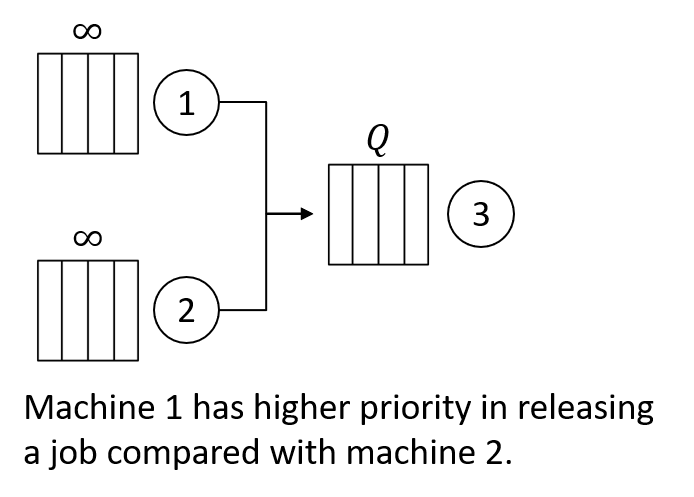
\includegraphics[width=0.4\textwidth]{Figures/merge.png}
	\caption{Example: single server merge.}
	\label{fig:merge}
\end{figure}

State variables have to be defined in the first place. Binary variable $w^{j}$ for $j=1,2,3$ equal to one represents if server $j$ is processing a job, otherwise it is equal to zero. Binary variable $b^{j}$ for $j=1,2$ equal to one represents if server $j$ is holding a finished job, otherwise it is equal to zero. State variable $b^3$ is not defined, since the job will be released immediately after its processing. Integer variable $q$ represents the number of jobs waiting in the buffer in front of server 3. 

The events composing the DES model are then defined as in Table \ref{tab:merge}. Event $e^{ss,j}$ for $j=1,2,3$ represents the starting of service of server $j$. If server $j$ is idle, i.e., neither working nor holding a finished part, $e^{ss,j}$ will be scheduled to execute immediately. After an $e^{ss,j}$ is executed, server $j$ works, i.e., state variable $g^j$ is incremented by one. Besides, if server 3 starts a job, the buffer level $q$ is decreased by one. Event $e^{d,j}$ for $j=1,2$ represents the departure of a job from server $j$. A $e^{d,1}$ can be executed if server 1 is holding a finished job and there is at least one space available in buffer 3. A $e^{d,2}$ can be executed immediately if server 2 is holding a finished job, server 2 is not holding a job and there is at least one space available in buffer 3. After executing $e^{d,j}$, the server is not holding any job, hence, state variable $b^{j}$ becomes zero, and the buffer level $q$ is increased by one. Both $e^{ss,j}$ and $e^{d,j}$ can executed immediately once scheduled, so they are zero-delay. Event $e^{f,j}$ represents that server $j$ finishes a job, and it is scheduled immediately after $e^{ss,j}$ is executed, and the delay until its execution is equal to the service time, i.e., a sample from $T^{j}$. Thus, $e^{ss,j}$ is a counting event of $e^{f,j}$. After event $e^{f,j}$ is executed, server $j$ is no longer working, thus, $g^j$ is decreased by one. Thus, state variable $g^j$ is a counting variable of $e^{f,j}$, since its value is incremented by one if $e^{ss,j}$ is executed, and decremented by one if  $e^{f,j}$ is executed. Specially for $j=1,2$, after a job is finished, the server holds a finished job, and state variable $b^j$ is increased by one. %If the simulation run includes $N^1$ jobs from server 1 and $N^2$ jobs from server 2, the number of executions of events $e^{ss,1}$, $e^{f,1}$, $e^{d,1}$ are equal to $N^1$, the number of executions of events $e^{ss,2}$, $e^{f,2}$, $e^{d,2}$ are equal to $N^2$, the number of executions of events $e^{ss,3}$, $e^{f,3}$ are equal to $N^1+N^2$.

\begin{table}[h]
	\begin{tabular}{lllllll} 
		\multicolumn{7}{l}{\textbf{Zero-delay events}}\\ \hline
		Variable&Event &  \multicolumn{4}{c}{Condition to schedule} & State change\\\hline
		$e^{ss,1}$ & Start m1 &  \multicolumn{4}{c}{$g^1\le 0\ \&\ b^1\le0 $} & $g^1${\footnotesize++} \\
		$e^{d,1}$&Depart m1&  \multicolumn{4}{c}{$b^1\ge1\ \&\  q\le Q-1$} &$b^1${\small-}{\small-}, $q${\footnotesize++} \\
		$e^{ss,2}$& Start m2 &  \multicolumn{4}{c}{$g^2\le 0\ \&\ b^2\le0 $} & $g^2${\footnotesize++} \\
		$e^{d,2}$&Depart m2&\multicolumn{4}{c}{$b^2\ge1\ \&\ q\le Q-1\ \&\ b^1\le 0$}&  $b^2${\small-}{\small-}, $q${\footnotesize++} \\
		$e^{ss,3}$ & Start m3 & \multicolumn{4}{c}{$g^3 \le 0\ \&\ q\ge 1$}&$g^3${\footnotesize++}, $q${\small-}{\small-} \\
		\multicolumn{7}{l}{\textbf{Positive-delay events}}\\ \hline
		Variable&Event 		   & Delay& $e^{\tilde{\xi}}$& $u^{\xi}$ &$\beta^{\xi}$& State change\\\hline
		$e^{f,1}$&Finish m1 & $T^{f,1}$& $e^{ss,1}$&  $g^1$&1&  $g^1${\small-}{\small-}, $b^1${\footnotesize++}\\	
		$e^{f,2}$&Finish m2 & $T^{f,2}$& $e^{ss,2}$&  $g^2$&1&  $g^2${\small-}{\small-}, $b^2${\footnotesize++}\\	
		$e^{f,3}$&Finish m3 & $T^{f,3}$& $e^{ss,3}$&  $g^3$&1&  $g^3${\small-}{\small-}\\	\hline
	\end{tabular}
	\caption{Events to simulate Single-server merge system.}
	\label{tab:merge}
\end{table}

The MPR proposed in this work is as follows: 
\begin{eqnarray}
(A1)-(A7),(B1),(B2),(B14),(B15),(B16)&& \forall \xi \in\{(ss,1),(ss,2),(ss,3),(d,1),(d,2)\}\nonumber\\
&&  \forall\xi \in\{(f,1),(f,2),(f,3)\}\nonumber\\
(B7),(B9)-(B12)&& \forall \xi \in\{(ss,1),(ss,2),(ss,3),(d,1),(d,2)\}\nonumber\\
%%%%%%%%%%%%%%%%%   \xi=(ss,1)(ss,2)   %%%%%%%%%%%%%%%%%%%%%%%%%%%
-u^{g^j}_k\ge z^{ss,j}_k-1&& \forall\ j=1,2,k\in \mathbb{K}\label{merge:ss1,1}\\
u^{g^j}_k\ge v^{ss,j,g^j,1}_k&& \forall\ j=1,2,k\in \mathbb{K}\label{merge:ss1,2}\\
-u^{b^j}_k\ge z^{ss,j}_k-1&& \forall\ j=1,2,k\in \mathbb{K}\label{merge:ss1,3}\\
u^{b^j}_k\ge v^{ss,j,b^j,1}_k&& \forall\ j=1,2,k\in \mathbb{K}\label{merge:ss1,4}\\
1-z^{ss,j}_k\le v^{ss,j,g^j,1}_k+v^{ss,j,b^j,1}_k+v^{ss,j,\beta}_k&& \forall\ j=1,2,k\in \mathbb{K}\label{merge:ss1,5}\\
%%%%%%%%%%%%%%%%%   \xi=(ss,3)   %%%%%%%%%%%%%%%%%%%%%%%%%%%
-u^{g^3}_k\ge z^{ss,3}_k-1&& \forall\ k\in \mathbb{K}\label{merge:ss3,1}\\
u^{g^3}_k\ge v^{ss,3,g^3,1}_k&& \forall\ k\in \mathbb{K}\label{merge:ss3,2}\\
u^{q}_k\ge z^{ss,3}_k&& \forall\ k\in \mathbb{K}\label{merge:ss3,3}\\
-u^{q}_k \ge Q(v^{ss,3,q,0}_k-1)&& \forall\ k\in \mathbb{K}\label{merge:ss3,4}\\
1-z^{ss,3}_k\le v^{ss,3,g^3,1}_k+v^{ss,3,q,0}_k+v^{ss,3,\beta}_k&& \forall\ k\in \mathbb{K}\label{merge:ss3,5}\\
%%%%%%%%%%%%%%%%%   \xi=(d,1)   %%%%%%%%%%%%%%%%%%%%%%%%%%%
u^{b^1}_k\ge z^{d,1}_k&& \forall\ k\in \mathbb{K}\label{merge:d1,1}\\
-u^{b^1}_k\ge v^{d,1,b^1,0}_k-1&& \forall\ k\in \mathbb{K}\label{merge:d1,2}\\
Q-u^{q}_k\ge z^{d,1}_k&& \forall\ k\in \mathbb{K}\label{merge:d1,3}\\
u^{q}_k\ge Qv^{d,1,q,1}_k&& \forall\ k\in \mathbb{K}\label{merge:d1,4}\\
1-z^{d,1}_k\le v^{d,1,b^1,0}_k+v^{d,1,q,1}_k+v^{d,1,\beta}_k&& \forall\ k\in \mathbb{K}\label{merge:d1,5}\\
%%%%%%%%%%%%%%%%%   \xi=(d,2)   %%%%%%%%%%%%%%%%%%%%%%%%%%%
u^{b^2}_k\ge z^{d,2}_k&& \forall\ k\in \mathbb{K}\label{merge:d2,1}\\
-u^{b^2}_k\ge v^{d,2,b^2,0}_k-1&& \forall\ k\in \mathbb{K}\label{merge:d2,2}\\
Q-u^{q}_k\ge z^{d,2}_k&& \forall\ k\in \mathbb{K}\label{merge:d2,3}\\
u^{q}_k\ge Qv^{d,2,q,1}_k&& \forall\ k\in \mathbb{K}\label{merge:d2,4}\\
-u^{b^1}_k\ge z^{d,2}_k-1&& \forall\ k\in \mathbb{K}\label{merge:d2,5}\\
u^{b^1}_k\ge v^{d,2,b^1,1}_k&& \forall\ k\in \mathbb{K}\label{merge:d2,6}\\
1-z^{d,2}_k\le v^{d,2,b^2,0}_k+v^{d,2,q,1}_k+v^{d,2,b^1,1}_k+v^{d,2,\beta}_k&& \forall\ k\in \mathbb{K}\label{merge:d2,7}
\end{eqnarray}
\begin{eqnarray}
%%%%%%%%%%%%%%%%%   \xi=(f,j)   %%%%%%%%%%%%%%%%%%%%%%%%%%%
x^{f,j}_{i,k} = w^{ss,j}_{i,k} && \forall\ j=1,2,3, i\in \mathbb{I}^{j},k\in \mathbb{K}\label{merge:f,1}\\
%%%%%%%%%%%%%%%%%   constraints E  %%%%%%%%%%%%%%%%%%%%%%%%%%% 
u^{g^j}_k=u^{g^j}_{k-1}+ \sum_{i\in\mathbb{I}^j}w^{ss,j}_{i,k}-\sum_{i\in\mathbb{I}^j}w^{f,j}_{i,k}&& \forall\ j=1,2,3, k\in \mathbb{K}\label{merge:E_wj}\\
u^{b^j}_k=u^{b^j}_{k-1}+ \sum_{i\in\mathbb{I}^j}w^{f,j}_{i,k}-\sum_{i\in\mathbb{I}^j}w^{d,j}_{i,k}&& \forall\ j=1,2, k\in \mathbb{K}\label{merge:E_bj}\\
u^{q}_k=u^{q}_{k-1}+\sum_{j=1,2}\sum_{i\in\mathbb{I}^j}w^{d,j}_{i,k}-\sum_{i\in\mathbb{I}^3}w^{ss,3}_{i,k}&& \forall\ k\in \mathbb{K}\label{merge:E_q}\\
%%%%%%%%%%%%%%%%%%%%%%%%%%%%%%%%%%%%%%%%%%%% 
u^{g^1}_0=u^{g^2}_0=u^{g^3}_0=u^{b^1}_0=u^{b^2}_0=u^{q}_0=0\nonumber\\
v^{ss,1,\beta}_0=v^{ss,2,\beta}_0=v^{ss,3,\beta}_0=v^{d,1,\beta}_0=v^{d,2,\beta}_0=0\nonumber\\
u^{g^1}_{k},u^{g^2}_{k},u^{g^3}_{k},u^{b^1}_{k},u^{b^2}_{k}\in\{0,1\},\ u^q_{k}\in\{0,...,Q\}&& \forall\ k\in \mathbb{K}\nonumber
\end{eqnarray}

Constraints (A1)-(A7) and (B1) (B2) (B14) (B15) (B16) are applied to all events. Events $e^{ss,j}$ for $j=1,2,3$ and $e^{d,j}$ for $j=1,2$ are all zero-delay, constraints (B3) to (B12) should be applied. Specifically, constraints (B7), (B9) to (B12) are identical for all systems, for sake of simplicity, they are not expanded. Constraints \eqref{merge:ss1,1} and \eqref{merge:ss1,3}, referring to constraints (B4), imply that if an execution of $e^{ss,j}$ is scheduled, machine $j$ is not occupied by a job under processing or a finished job. Constraints \eqref{merge:ss1,2} and \eqref{merge:ss1,4}, referring to constraints (B6), imply that if variable $v^{ss,j,g^j,1}_k$ or $v^{ss,j,b^j,1}_k$ is equal to one, machine $j$ is occupied by a job under processing or a finished job. Constraints \eqref{merge:ss1,5}, referring to constraints (B8), state that if event $e^{ss,1}$ or $e^{ss,2}$ is not scheduled, it is either the machine is occupied, or there is already an execution in the future event list. Similarly, constraints \eqref{merge:ss3,1} to \eqref{merge:ss3,5} refer to constraints (B3) to (B6) and (B8) of event $e^{ss,3}$, stating that an execution of event $e^{ss,3}$ can be scheduled if and only if machine 3 is not occupied, there is a job waiting in buffer 3, there is no executions of $e^{ss,3}$ in the future event list. Constraints \eqref{merge:d1,1} to \eqref{merge:d1,5} refer to constraints (B3) to (B6) and (B8) of event $e^{d,1}$, implying that an execution of event $e^{d,1}$ can be scheduled if and only if there is a finished job in machine 1, there is space available in buffer 3, there is no executions of $e^{d,1}$ in the future event list. Constraints \eqref{merge:d2,1} to \eqref{merge:d2,7} refer to constraints (B3) to (B6) and (B8) of event $e^{d,2}$, depicting that an execution of event $e^{d,2}$ can be scheduled if and only if there is a finished job in machine 2, there is space available in buffer 3, there is no finished job waiting in machine 1, there is no executions of $e^{d,2}$ in the future event list. Since events $e^{f,j}$ are positive-delay, constraints (B13) should be applied, as in constraints \eqref{merge:f,1}. A finishing event of machine $j$ can be scheduled after a starting event is executed. Constraints \eqref{merge:E_wj} to \eqref{merge:E_q} indicate the evolution of state variables $g^j$, $b^j$ and $q$, respectively. $g^j$ is increased by one if machine $j$ starts a job and decreased by one if it finished a job. $b^j$ is increased by one if machine $j$ finishes a job, and decreased by one if it releases a job. $q$ is increased by one if machine 1 or 2 releases a job, and decreased by one if machine 3 seizes a job from buffer 3.


\subsection{G/G/1 with failure}
A G/G/1 queueing system with unreliable server is studied in this section. The server has two state, up and down, respectively. When the server is in up state, it can process a job. When the server turns to down state from up state, the repair starts immediately, and if the server is processing a job, the job is discarded. After the repair finishes, the server turns to up state, and restarts to process jobs. The repair time follows a general distribution. The server will then keep in up state for a certain time called up time, following a general distribution, and will fail again. The failure is time-dependent. Jobs arrive at the system following a general arrival process and enter the queue in front of the server. When the server is in up state and idle, the server can take a job from the queue and start the service. After the service, a job can be released from the system immediately.

The state variables include integer variable $q$ representing the number of jobs in the queue, binary variable $w$ indicating whether the server is working or not, binary variable $h$ indicating whether the server is in down state or not, and binary variable $r$ representing whether the server is under repair.

The events composing the DES model are then defined as in Table \ref{tab:failure}. Event $e^{arr}$ indicates that a job arrives at the system, and it is scheduled after a previous arrival, with a delay equal to the inter-arrival time. A counting event of $e^{arr}$, i.e., $e^{\tilde{arr}}$, and a counting variable $u^{arr}$ should be defined. The condition to schedule an arrival is that there is no execution of $e^{arr}$ in the future event list. When $e^{\tilde{arr}}$ is executed, the counting variable $u^{arr}$, i.e., the number of executions of $e^{arr}$ in the future event list will be increased by one. When $e^{arr}$ is executed, the number of jobs in the queue will be increased by one, and the counting variable $u^{arr}$ will be decreased by one. Event $e^{ss}$ represents that the server starts to process a job. If and only if there is at least one job in the queue, the server is in upstate and idle, event $e^{ss}$ is scheduled. When event $e^{ss}$ is executed, the number of jobs in the queue is reduced by one, and the server starts to work, i.e., state variable $w$ becomes to one. Event $e^{f}$ represents that a server finishes a job, and it is scheduled after each execution of start with a delay equal to service time. Event $e^{ss}$ is the counting event, and state variable $w$ is the counting variable of $e^{f}$. After $e^{f}$ is executed, the server becomes idle. Once the server is in down state, job under process is discarded, i.e., scheduled execution of $e^{f}$ is canceled. Event $e^{fl}$ represents that the state of the server becomes down, and it is scheduled after the previous repair finishes with delay equal to up time. Since it is positive-delay, a count event $e^{\tilde{fl}}$ should be added, and also a counting variable $u^{fl}$. The condition to scheduled an $e^{\tilde{fl}}$ is that the the server is in up state, i.e., $h$ equal to zero, and there is no execution of $e^{fl}$ in the future event list, i.e., $u^{fl}$ smaller or equal to zero. When $e^{\tilde{fl}}$ is executed, the number of executions of $e^{fl}$ is increased by one. When $e^{fl}$ is executed, the server is in down state, it cannot be working, i.e., $w$ equal to zero, and the number of executions in the future event list of itself is reduced by one. Event $e^{srp}$ represents start of repair, and it is scheduled if the server is in down state and not under repair, and executed with no delay. When it is executed, the server is under repair. Event $e^{frp}$ states the finish of repair, and it is scheduled after event $e^{srp}$ is executed, hence, $e^{srp}$ is the counting event, and state variable $r$ can be used as the counting variable. After it is executed, the server becomes up, and no longer under repair. %If the simulation included $N$ arrivals and $N^{fl}$ failures, the number of executions of $e^{\tilde{arr}}$, $e^{ss}$, $e^{arr}$ and $e^{f}$ is equal to $N$, and the number of executions of $e^{\tilde{fl}}$, $e^{srp}$, $e^{fl}$ and $e^{frp}$ is equal to $N^{fl}$.

\begin{table}[h]
	\begin{tabular}{llllllll} 
		\multicolumn{8}{l}{\textbf{Zero-delay events}}\\ \hline
		Variable&Event &  \multicolumn{4}{c}{Condition to schedule} & State change&\\\hline
		$e^{\tilde{arr}}$ & Count arrival &  \multicolumn{4}{c}{$u^{arr}\le 0$} & $u^{arr}${\footnotesize++}& \\
		$e^{ss}$&Start&  \multicolumn{4}{c}{$1\le q,\ g\le 0,\ h\le 0$} &$g${\footnotesize++}, $q${\small-}{\small-}&  \\
		$e^{\tilde{fl}}$& Count failure &  \multicolumn{4}{c}{$h\le 0,\ u^{fl}\le 0$} & $u^{fl}${\footnotesize++}& \\
		$e^{srp}$&Start to repair&\multicolumn{4}{c}{$h\ge 1,\ r\le 0$}&  $r${\footnotesize++}&  \\
		\multicolumn{8}{l}{\textbf{Positive-delay events}}\\ \hline
		Variable&Event 		   & Delay& $e^{\tilde{\xi}}$& $u^{\xi}$ &$\beta^{\xi}$& State change&Condition \\
		&&&&&&&to cancel\\\hline
		$e^{arr}$&Arrival & $T^{arr}$& $e^{\tilde{arr}}$&  $u^{arr}$&1&  $u^{arr}${\small-}{\small-},  $q${\footnotesize++}&\\	
		$e^{f}$&Finish & $T^{f}$& $e^{ss}$&  $g$&1&  $g${\small-}{\small-}&$h\ge 1$, $g\ge 1$\\	
		$e^{fl}$&Failure & $T^{fl}$& $e^{\tilde{fl}}$&  $u^{fl}$&1&   $h${\footnotesize++}, $u^{fl}${\small-}{\small-}&\\	
		$e^{frp}$&Finish of repair & $T^{rp}$& $e^{srp}$&  $r$&1&   $h${\small-}{\small-}, $r${\small-}{\small-}&\\	\hline
	\end{tabular}
	\caption{Events to simulate G/G/1 with failure.}
	\label{tab:failure}
\end{table}


The MPR proposed in this work is as follows.

\begin{eqnarray}
(A1)-(A7),(B1),(B2),(B15),(B16),(B17)&& \forall \xi \in\{\tilde{arr},ss,\tilde{fl},srp\}\nonumber\\
&&  \forall\xi \in\{arr,f,fl,frp\}\nonumber\\
(B3)-(B13)&& \forall \xi \in\{\tilde{arr},ss,\tilde{fl},srp\}\nonumber\\
(B14)&& \forall\xi \in\{arr,f,fl,frp\}\nonumber\\
u^{h}_k\ge z^{\bar{f}}_k&&\forall\ k\in \mathbb{K}\label{fail:D1}\\
-u^{h}_k\ge v^{\bar{f},h,0}_k-1&&\forall\ k\in \mathbb{K}\label{fail:D2}\\
u^{g}_{k-1}\ge z^{\bar{f}}_k &&\forall\ k\in \mathbb{K}\label{fail:D3}\\
-u^{g}_{k-1} \ge v^{\bar{f},g,0}_k-1&&\forall\ k\in \mathbb{K}\label{fail:D4}\\
1-z^{\bar{f}}_k\le v^{\bar{f},s,0}_k+v^{\bar{f},g,0}_k&&\forall\ k\in \mathbb{K}\label{fail:D5}\\
k^{f,1}_i=\sum_{k\in\mathbb{K}}kw^{f}_{k,i}&&\forall\ i\in \mathbb{I}^{\xi}\label{fail:D6}\\
k^{f,0}_i=\sum_{k\in\mathbb{K}}kx^{f}_{k,i}&&\forall\ i\in \mathbb{I}^{\xi}\label{fail:D7}\\
kz^{\bar{f}}_k -k^{f,0}_i - 1 \ge K(\theta^{f}_{i,k}-1)&&\forall\ i\in \mathbb{I}^{\xi},k\in \mathbb{K}\label{fail:D8}\\
k^{f,1}_i - 1 - kz^{\bar{f}}_k \ge k(\theta^{f}_{i,k}-1)&&\forall\  i\in \mathbb{I}^{\xi},k\in \mathbb{K}\label{fail:D9}\\
k^{f,0}_i - kz^{\bar{f}}_k \ge k(\phi^{f,0}_{i,k}-1)&&\forall\ i\in \mathbb{I}^{\xi},k\in \mathbb{K}\label{fail:D10}\\
kz^{\bar{f}}_k - k^{f,1}_i \ge K(\phi^{f,1}_{i,k}-1)&&\forall\ i\in \mathbb{I}^{\xi},k\in \mathbb{K}\label{fail:D11}\\
1-\theta^{f}_{i,k} \le \phi^{f,0}_{i,k} + \phi^{f,1}_{i,k}&&\forall\ i\in \mathbb{I}^{\xi},k\in \mathbb{K}\label{fail:D12}\\
\gamma^{f}_{i,k} \ge w^{f}_{i,k} - \sum_{k^{'}\in \mathbb{K}}\theta^{f}_{i,k^{'}}&&\forall\ i\in \mathbb{I}^{\xi},k\in \mathbb{K}\label{fail:D13}\\
w^{f}_{i,k} - \sum_{k^{'}\in \mathbb{K}}\theta^{f}_{i,k^{'}} -1 \ge (N^{fl}+1)(\gamma^{f}_{i,k}-1) &&\forall\ i\in \mathbb{I}^{\xi},k\in \mathbb{K}\label{fail:D14}
\end{eqnarray}
\begin{eqnarray}
u^{arr}_k=u^{arr}_{k-1}+ \sum_{i\in\mathbb{I}^j}w^{\tilde{arr}}_{i,k}-\sum_{i\in\mathbb{I}^j}w^{arr}_{i,k}&&\forall\ k\in \mathbb{K}\label{fail:E1}\\
u^{q}_k=u^{q}_{k-1}+ \sum_{i\in\mathbb{I}^j}w^{arr}_{i,k}-\sum_{i\in\mathbb{I}^j}w^{ss}_{i,k}&&\forall\ k\in \mathbb{K}\label{fail:E2}\\
u^{fl}_k=u^{fl}_{k-1}+ \sum_{i\in\mathbb{I}^j}w^{\tilde{fl}}_{i,k}-\sum_{i\in\mathbb{I}^j}w^{fl}_{i,k}&&\forall\ k\in \mathbb{K}\label{fail:E3}\\
u^{r}_k=u^{r}_{k-1}+ \sum_{i\in\mathbb{I}^j}w^{srp}_{i,k}-\sum_{i\in\mathbb{I}^j}w^{frp}_{i,k}&&\forall\ k\in \mathbb{K}\label{fail:E4}\\
u^{g}_k \le 1-z^{\bar{f}}_{k}&&\forall\ k\in \mathbb{K}\label{fail:E5}\\
u^{g}_k\le u^{g}_{k-1}- \sum_{i\in \mathbb{I}} \gamma^{f}_{i,k} +\sum_{i\in \mathbb{I}} w^{ss}_{i,k} + z^{\bar{f}}_{k}&&\forall\ k\in \mathbb{K}\label{fail:E6}\\
u^{g}_k\ge u^{g}_{k-1}-  \sum_{i\in \mathbb{I}} \gamma^{f}_{i,k} +\sum_{i\in \mathbb{I}} w^{ss}_{i,k}  - z^{\bar{f}}_{k}&&\forall\ k\in \mathbb{K}\label{fail:E7}\\
u^{arr}_0=u^{fl}_0=u^{r}_0=u^{g}_0=u^{q}_0=0\nonumber\\
v^{\xi,\beta}_0=0&& \forall \xi \in\{\tilde{arr},ss,\tilde{fl},srp\}\nonumber\\
u^{arr}_k,u^{fl}_k,u^{r}_k,u^{g}_k\in\{0,1\},\ u^{q}_k\in\{0,...,Q\}\nonumber
\end{eqnarray}
Constraints (A1)-(A7) and (B1) (B2) are applied to all events. Events $e^{\tilde{arr}}$, $e^{ss}$, $e^{\tilde{fl}}$ and $e^{srp}$ are all zero-delay, constraints (B3) to (B13) should be applied, and constraints (B14) should be applied to events $e^{arr}$, $e^{f}$, $e^{fl}$ and $e^{frp}$. The group-B constraints have been explained in previous two examples, this example will not expand them. Constraints \eqref{fail:D1} to \eqref{fail:D14} are group-C constraints for canceling event $e^{f}$. Binary variable $z^{\bar{f}}_k$ equal to one represents that execution of $e^{f}$ is removed from the future event list, otherwise the execution is not canceled. Specifically, constraints \eqref{fail:D1} and \eqref{fail:D3} show that if $e^{f}$ is canceled, state variable $h$ must be greater than or equal to one, and there is at one execution of $f$ in the future event list. Constraints \eqref{fail:D2} indicate that if $v^{\bar{f},h,0}$ is equal to one, the cancellation condition is violated. Constraints \eqref{fail:D4} indicate that if $v^{\bar{f},\beta}$ is equal to one, there is no executions of $e^{f}$ in the future event list. Constraints \eqref{fail:D5} show that if execution of $e^{f}$ is not canceled, i.e., $z^{\bar{f}}_k$ equal to zero, it is either that the cancellation condition is false or there is no execution in the event list. Integer variables $k^{f,0}_i$ denote the index of overall execution $\mathcal{E}$ that scheduled the $i$-th execution of $e^{f}$, and $k^{f,1}_i$ denotes the execution index of the the $i$-th execution of $e^{f}$, as in constraints \eqref{fail:D6} and \eqref{fail:D7}. Binary variable $\theta^{f}_{i,k}$ equal to one represents that the $i$-th execution of $e^{f}$ is canceled after execution $\mathcal{E}_k$. Constraints \eqref{fail:D8} and \eqref{fail:D9} state that if the $i$-th execution of $e^{f}$ is canceled after execution $\mathcal{E}_k$, then it must be scheduled before $\mathcal{E}_k$ and executed after $\mathcal{E}_k$. Binary variable $\phi^{f,0}_{i,k}$ equal to one indicates that the condition to cancel $e^{f}$ is not true after execution $\mathcal{E}_k$ or the $i$-th execution of $e^{f}$ is scheduled after $\mathcal{E}_k$, as in constraints \eqref{fail:D10}. Binary variable $\phi^{f,1}_{i,k}$ equal to one indicates that the $i$-th execution of $e^{f}$ is executed before $\mathcal{E}_k$, as in constraints \eqref{fail:D11}. Constraints \eqref{fail:D12} state that if execution $i$ of $e^{f}$ is not canceled after execution $\mathcal{E}_k$, it is either because the condition to cancel to false, or it is executed before $\mathcal{E}_k$ or it is scheduled after $\mathcal{E}_k$. Binary variable $\gamma^{f}_{i,k}$ equal to one represents that the $k$-th execution $\mathcal{E}_k$ is an event $e^{f}$ and it eventually change the system state, as in constraints \eqref{fail:D14}. Constraints \eqref{fail:D13} state that if $\gamma^{f}_{i,k}$ is equal to zero, it is either because execution $\mathcal{E}_k$ is not the $i$-th execution of event $e^{f}$ or it is canceled. Constraints \eqref{fail:E1} to \eqref{fail:E7} depict the evolution of state variables. Constraints \eqref{fail:E1} to \eqref{fail:E4}, referring to constraints (E5) and (E6), are similar to the two examples above, state variables $arr$, $q$, $fl$ and $r$ are all changed by events without cancellation. Constraints \eqref{fail:E5} state that if event $e^{f}$ is canceled after execution $\mathcal{E}_k$, the number of executions of $e^{f}$ in the future event list will be reduced to zero. Constraints \eqref{fail:E6} and \eqref{fail:E7} show that if $e^{f}$ is not canceled by execution $\mathcal{E}_k$, the state variable $w$ will be increased by one if $e^{ss}$ is executed, and decreased by one if $e^{f}$ is executed without being canceled.



\section{Discussion}\label{sec:discussion}

This work proposes an MPR of DES model that satisfies certain assumptions, based on the widely-applied event-scheduling execution logic of DES. In the MPR, the decision variables include event scheduling time, execution time, and system state after each event execution, and the constraints represent that events are scheduled or canceled when the system state satisfies the condition to schedule or cancel. Furthermore, the MPR also takes the samples of random variables as the coefficients of constraints, where the random variate are usually the time delay between the execution time and scheduled time of events. Thus, the MPR represents a sample path of the DES. However, expanding the MPR from single-sample-path model into a multiple-sample-path model can be achieved by add one more subscripts to each decision variables, and the resulting MPR is separable since there is not constraints linking variables from distinguished sample paths, i.e., the sample paths are independent from each other. 

The MPR proposed in this work differs from the state-of-the-art MPR \citep{chan2008optimization} in objective function. In the state-of-the-art formulation, the constraints represent the event triggering relationships, i.e., the execution time of the triggered event must be later than that of the triggering event with a delay, which is a sample from predefined random variate. Hence, the objective function must be the minimization of the execution time of all the events, so that all the events are executed as soon as possible. In this work, the constraints represent that once the condition to schedule or cancel an event is true, the event must be scheduled or canceled, i.e., the logic that events must be executed as soon as possible is forced by constraints. Thus, the objective function can be defined in a more flexible way. 

The representation of event cancellation is presented in this work, which has never been studied in literature. This contribution extends the application of MPR, as in section 3.3.

As can be seen, the proposed MPR contains both integer variables and real-valued variables. If the steady state performance from simulation model is of interest, the simulation length, i.e., the number of event executions, is usually long. Thus, the MPR is with many variables and constraints. Generally speaking, it is reasonable to using the MPR as an representation instead of solving it as an MPR as the computational complexity is extremely high. An application of the MPR is the calculation sub-gradient from a simulation run, based on the sensitivity analysis of the approximate linear programming (LP) of the MPR. The procedure is as follows. The DES is first simulated with an event-scheduling execution logic, and the values of all decision variables of the MPR can be obtained during the simulation run. We formulate the approximate LP by replacing all the decision variables with a big-M multiplier, i.e., all variables except the once representing event scheduling time, execution time, and state variables, with its value obtained from the simulation, and relaxing the integrality of remaining variables. By solving the dual problem of the approximate LP, we can get the gradient of objective function on some coefficients, for instance, the thresholds $a^{\xi}_s$ and $c^{\xi}_s$ of inequalities, which are part of the conditions to schedule events. Another way to make use of the MPR is to deriving an MPR of a simulation optimization problem. In the application in manufacturing and service operation, the decision variables of an optimization problem are usually the thresholds $a^{\xi}_s$ and $c^{\xi}_s$ of inequalities, which are part of the conditions to schedule events. So, to transform the MPR of simulation into MPR of simulation optimization, one just need to specify that certain thresholds are decision variables instead of coefficients. Then, the system performance could be in the objective function or in a constraint stating that it has to achieve a target. The convenience of transforming the proposed MPR into an MPR of simulation optimization represents another contribution of this work. However, the resulting MPR still has computational issue, which leads to our future research interest.

\newpage
\section*{Appendix I: G/G/m of Chan \& Schruben's model}

The MPR model proposed in \cite{chan2008optimization} is as follows:
\begin{eqnarray}
\min\{\sum_{i=1}^N (e^{a}_{i,1}+e^{r}_{i,1}+e^{f}_{i,1})\}\nonumber\\
e^{a}_{i,1} - e^{a}_{i-1,1} = t^{a}_{i}&&\forall\ i \label{GG1erg:1}\\
e^{f}_{j,1} - e^{r}_{i,1} \ge t^{f}_{i}-M(1-\sum_{l=max\{i-m+1,1\}}^{j} y^{f}_{i,l})&&\forall\ i,j\label{GG1erg:2}\\
e^{r}_{i,1} - e^{a}_{i,1} \ge 0&&\forall\ i\label{GG1erg:3}\\
e^{r}_{i,1} - e^{f}_{i-m,1} \ge 0&&\forall\ i\label{GG1erg:4}\\
\sum_{l=max\{i-m+1,1\}}^n y^{f}_{i,l} = 1 && \forall i\\
\sum_{i=1}^{min\{j+m-1,n\}} y^{f}_{i,l} = 1 && \forall j
\end{eqnarray}

To explain the MPR model, the ERG of G/G/1 queue is first shown in Figure \ref{fig:ERG_GG1}. Each triggering relationship in the ERG, i.e., two connected nodes is represented by one constraint. Constraints \eqref{GG1erg:1} to \eqref{GG1erg:4} state the relationships of $e^a \rightarrow e^a$, $e^s\rightarrow e^f$, $e^a\rightarrow e^s$ and $e^f\rightarrow e^s$, respectively. The objective function is the sum of all the event execution time. As can be seen, the model is a linear programming. 

\begin{figure}[h]
	\centering
	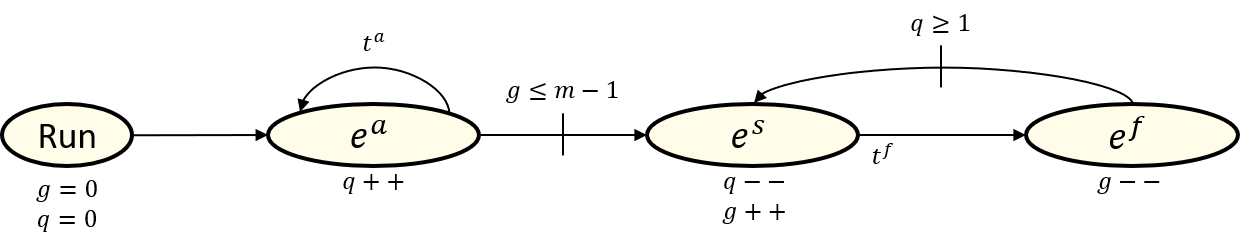
\includegraphics[width=0.7\textwidth]{Figures/ERG_GG1.png}
	\caption{ERG of G/G/1 queue.}
	\label{fig:ERG_GG1}
\end{figure}

\section*{Appendix II: single-server merge of Chan \& Schruben's model}

The MPR model proposed in \cite{chan2008optimization} is as follows:

\begin{eqnarray}
\min\{\sum_{i=1}^{N_1} (e^{s,1}_i+e^{f,1}_{i}+e^{d,1}_{i})+\sum_{i=1}^{N_2}(e^{s,2}_i+e^{f,2}_{i}+e^{d,2}_{i}) + \sum_{i}^{} e^{d,2,1}_{i}+\nonumber\\
\sum_{i=1}^{N_1+N_2}(e^{s,3}_i+e^{d,3}_{i}-e^{w:(d,1),(d,2)}_i) +\sum_{i=1}^{N_1+N_2}\sum_{k=1}^{N_1} e^{p:(d,1),(d,2)}_{i,k,i-k}\}\nonumber\\
e^{s,1}_i - e^{d,1}_{i-1} = 0\label{MergeErg:1} \\
e^{f,1}_{i} - e^{s,1}_{i} = t^{1}_i\\
e^{s,2}_i - e^{d,2}_{i-1} = 0\\
e^{f,2}_{i} - e^{s,2}_{i} = t^{2}_i\\
%e^{d,2,1}_{i} - e^{f,2}_{i} \ge 0\\
e^{d,3}_{i} - e^{s,3}_{i} = t^{3}_i\\
e^{d,1}_{i} - e^{f,1}_{i} \ge 0\label{MergeErg:6} \\
e^{s,3}_{i} - e^{d,3}_{i-1} \ge 0\label{MergeErg:7} 
\end{eqnarray}


%%%%%%%%%%%%%%%% e^{d,2,1}_j -> e^{d,2}_i   【Case D】 %%%%%%%%%%%%%%%%%%%%%%%%%%%%%%%%%%%
\begin{eqnarray}
e^{d,2}_i-e^{d,2,1}_j\ge M(\sigma_{(d,2,1):j,(d,2):i}-1)\label{MergeErg:8.1}\\
e^{d,2}_i-e^{d,2,1}_j\ge m(1 - \sigma_{(d,2,1):j,(d,2):i})\\
e^{d,2,1}_{j} \ge e^{d,1}_{k} - M(1-\zeta_{(d,1):k,(d,2,1):j})\\ 
e^{d,1}_{k} \ge e^{d,2,1}_{j} + m\zeta_{(d,1):k,(d,2,1):j} +(1-\zeta_{(d,1):k,(d,2,1):j})\varepsilon\\ 
e^{f,1}_{k+1} \ge e^{d,2,1}_{j} - M(1-\eta_{(d,2,1):j,(f,1):k+1})\\
e^{d,2,1}_{j} \ge e^{f,1}_{k+1} + m\eta_{(d,2,1):j,(f,1):k+1}\\
\gamma_{(d,1):k,(d,2,1):j} - (\zeta_{(d,1):k,(d,2,1):j} + \eta_{(d,2,1):j,(f,1):k+1})+1\ge 0\\
2\gamma_{(d,1):k,(d,2,1):j}-(\zeta_{(d,1):k,(d,2,1):j} + \eta_{(d,2,1):j,(f,1):k+1})\le 0\\
\sum_k\gamma_{(d,1):k,(d,2,1):j}-\sum_i \sigma_{(d,2,1):j,(d,2):i} \ge 0\\
n\sum_{i}\sigma_{(d,2,1):j,(d,2):i} - \sum_k\gamma_{(d,1):k,(d,2,1):j}\ge 0\\
\sum_{i}\sigma_{(d,2,1):j,(d,2):i}\le 1\\
\sum_{j}\sigma_{(d,2,1):j,(d,2):i}\le 1\\
\sum_{j=i}^{n}\sigma_{(d,2,1):j,(d,2):i}\ge \sum_{j=i+1}^{n}\sigma_{(d,2,1):j,(d,2):i+1}\\
\sum_{p=j+1}^n\sum_{q=1}^{i-1} \sigma_{(d,2,1):p,(d,2):q} \ge min\{i-1,n-j\}(1-\sigma_{(d,2,1):j,(d,2):i})\label{MergeErg:8.2}
\end{eqnarray}


%%%%%%%%%%%%%%%% e^{d,3}_j -> e^{d,2,1}_i   【Case D】 %%%%%%%%%%%%%%%%%%%%%%%%%%%%%%%%%%%
\begin{eqnarray}
e^{d,2,1}_i-e^{s,3}_j\ge M(\sigma_{(s,3):j,(d,2,1):i}-1)\label{MergeErg:9.1}\\
e^{d,2,1}_i-e^{s,3}_j\ge m(1 - \sigma_{(s,3):j,(d,2,1):i})\\
e^{s,3}_{j} \ge e^{f,2}_{k} - M(1-\zeta_{(f,2):k,(s,3):j})\\ 
e^{f,2}_{k} \ge e^{s,3}_{j} + m\zeta_{(f,2):k,(s,3):j} +(1-\zeta_{(f,2):k,(s,3):j})\varepsilon\\ 
e^{d,2}_{k+1} \ge e^{s,3}_{j} - M(1-\eta_{(s,3):j,(d,2):k+1})\\
e^{s,3}_{j} \ge e^{d,2}_{k+1} + m\eta_{(s,3):j,(d,2):k+1}\\
\gamma_{(f,2):k,(s,3):j} - (\zeta_{(f,2):k,(s,3):j} + \eta_{(s,3):j,(d,2):k+1})+1\ge 0\\
2\gamma_{(f,2):k,(s,3):j}-(\zeta_{(f,2):k,(s,3):j} + \eta_{(s,3):j,(d,2):k+1})\le 0\\
\sum_k\gamma_{(f,2):k,(s,3):j}-\sum_i \sigma_{(s,3):j,(d,2,1):i} \ge 0\\
n\sum_{i}\sigma_{(s,3):j,(d,2,1):i} - \sum_k\gamma_{(f,2):k,(s,3):j}\ge 0\\
\sum_{i}\sigma_{(s,3):j,(d,2,1):i}\le 1\\
\sum_{j}\sigma_{(s,3):j,(d,2,1):i}\le 1\\
\sum_{j=i}^{n}\sigma_{(s,3):j,(d,2,1):i}\ge \sum_{j=i+1}^{n}\sigma_{(s,3):j,(d,2,1):i+1}\\
\sum_{p=j+1}^n\sum_{q=1}^{i-1} \sigma_{(s,3):p,(d,2,1):q} \ge min\{i-1,n-j\}(1-\sigma_{(s,3):j,(d,2,1):i})\label{MergeErg:9.2}
\end{eqnarray}


%%%%%%%%%%%%%%%% 【Convolution】  e^{d,1} & e^{d,2} %%%%%%%%%%%%%%%%%%%%%%%%%%%%%%%%%%%
\begin{eqnarray}
e^{w:(d,1),(d,2)}_i\le e^{p:(d,1),(d,2)}_{i,k,i-k}\label{MergeErg:10.1}\\
e^{d,1}_k\ge e^{d,2}_{i-k} - M(1-\alpha^{(d,1),(d,2)}_{i,k,i-k})\\
e^{d,2}_{i-k} \ge e^{d,1}_{i-k} + m\alpha^{(d,1),(d,2)}_{i,k,i-k}+(1-\alpha^{(d,1),(d,2)}_{i,k,i-k})\varepsilon\\
e^{p:(d,1),(d,2)}_{i,k,i-k}\ge e^{d,1}_k - M(1-\alpha^{(d,1),(d,2)}_{i,k,i-k})\\
e^{d,1}_k\ge e^{p:(d,1),(d,2)}_{i,k,i-k}+m(1-\alpha^{(d,1),(d,2)}_{i,k,i-k})\\
e^{p:(d,1),(d,2)}_{i,k,i-k}\ge e^{d,2}_k - M\alpha^{(d,1),(d,2)}_{i,k,i-k}\\
e^{d,2}_k\ge e^{p:(d,1),(d,2)}_{i,k,i-k}+m\alpha^{(d,1),(d,2)}_{i,k,i-k}\label{MergeErg:10.2}
\end{eqnarray}


%%%%%%%%%%%%%%%% e^{f,2}_j -> e^{d,2,1}_i   【Case (h)】 %%%%%%%%%%%%%%%%%%%%%%%%%%%%%%%%%%%
\begin{eqnarray}
e^{d,2,1}_i-e^{f,2}_j\ge M(\sigma_{(f,2):j,(d,2,1):i}-1)\label{MergeErg:11.1}\\
e^{d,2,1}_i-e^{f,2}_j\ge m(1 - \sigma_{(f,2):j,(d,2,1):i})\\
e^{f,2}_{j} \ge e^{s,3}_{k} - M(1-\zeta_{(s,3):k,(f,2):j})\\ 
e^{s,3}_{k} \ge e^{f,2}_{j} + m\zeta_{(s,3):k,(f,2):j} +(1-\zeta_{(s,3):k,(f,2):j})\varepsilon\\ 
e^{w:(d,1),(d,2)}_{k+Q} \ge e^{f,2}_{j} - M(1-\eta_{(f,2):j,(w:(d,1),(d,2)):k+Q})\\
e^{f,2}_{j} \ge e^{w:(d,1),(d,2)}_{k+Q} + m\eta_{(f,2):j,(w:(d,1),(d,2)):k+Q}\\
\gamma_{(s,3):k,(f,2):j} - (\zeta_{(s,3):k,(f,2):j} + \eta_{(f,2):j,(w:(d,1),(d,2)):k+Q})+1\ge 0\\
2\gamma_{(s,3):k,(f,2):j}-(\zeta_{(s,3):k,(f,2):j} + \eta_{(f,2):j,(w:(d,1),(d,2)):k+Q})\le 0\\
\sum_k\gamma_{(s,3):k,(f,2):j}-\sum_i \sigma_{(f,2):j,(d,2,1):i} \ge 0\\
n\sum_{i}\sigma_{(f,2):j,(d,2,1):i} - \sum_k\gamma_{(s,3):k,(f,2):j}\ge 0\\
\sum_{i}\sigma_{(f,2):j,(d,2,1):i}\le 1\\
\sum_{j}\sigma_{(f,2):j,(d,2,1):i}\le 1\\
\sum_{j=i}^{n}\sigma_{(f,2):j,(d,2,1):i}\ge \sum_{j=i+1}^{n}\sigma_{(f,2):j,(d,2,1):i+1}\\
\sum_{p=j+1}^n\sum_{q=1}^{i-1} \sigma_{(f,2):p,(d,2,1):q} \ge min\{i-1,n-j\}(1-\sigma_{(f,2):j,(d,2,1):i})\label{MergeErg:11.2}
\end{eqnarray}

%%%%%%%%%%%%%%%% e^{d,3}_j -> e^{s,3}_i   【Case (f)】 %%%%%%%%%%%%%%%%%%%%%%%%%%%%%%%%%%%
\begin{eqnarray}
e^{s,3}_i \ge e^{w:(d,1),(d,2)}_{i}\label{MergeErg:12}
\end{eqnarray}

\begin{eqnarray}
%%%%%%%%%%%%%%%% e^{f,1}_j -> e^{d,1}_i   【Case (f)】 %%%%%%%%%%%%%%%%%%%%%%%%%%%%%%%%%%%
e^{d,1}_i-e^{f,1}_j\ge M(\sigma_{(f,1):j,(d,1):i}-1)\label{MergeErg:13.1}\\
e^{d,1}_i-e^{f,1}_j\ge m(1 - \sigma_{(f,1):j,(d,1):i})\\
e^{f,1}_{j} \ge e^{s,3}_{k} - M(1-\zeta_{(s,3):k,(f,1):j})\\ 
e^{s,3}_{k} \ge e^{f,1}_{j} + m\zeta_{(s,3):k,(f,1):j} +(1-\zeta_{(s,3):k,(f,1):j})\varepsilon\\ 
e^{d,2}_{k+Q} \ge e^{f,1}_{j} - M(1-\eta_{(f,1):j,(d,2):k+Q})\\
e^{f,1}_{j} \ge e^{d,2}_{k+Q} + m\eta_{(f,1):j,(d,2):k+Q}\\
\gamma_{(s,3):k,(f,1):j} - (\zeta_{(s,3):k,(f,1):j} + \eta_{(f,1):j,(d,2):k+Q})+1\ge 0\\
2\gamma_{(s,3):k,(f,1):j}-(\zeta_{(s,3):k,(f,1):j} + \eta_{(f,1):j,(d,2):k+Q})\le 0\\
\sum_k\gamma_{(s,3):k,(f,1):j}-\sum_i \sigma_{(f,1):j,(d,1):i} \ge 0\\
n\sum_{i}\sigma_{(f,1):j,(d,1):i} - \sum_k\gamma_{(s,3):k,(f,1):j}\ge 0\\
\sum_{i}\sigma_{(f,1):j,(d,1):i}\le 1\\
\sum_{j}\sigma_{(f,1):j,(d,1):i}\le 1\\
\sum_{j=i}^{n}\sigma_{(f,1):j,(d,1):i}\ge \sum_{j=i+1}^{n}\sigma_{(f,1):j,(d,1):i+1}\\
\sum_{p=j+1}^n\sum_{q=1}^{i-1} \sigma_{(f,1):p,(d,1):q} \ge min\{i-1,n-j\}(1-\sigma_{(f,1):j,(d,1):i})\label{MergeErg:13.2}
\end{eqnarray}

To explain the MPR model, the ERG of the merge system is first shown in Figure \ref{fig:ERG_merge}. Each triggering relationship in the ERG is represented by one or more constraints. Since the modeling framework requires that there is at most one condition on each arc, event $e^{d,2,1}$ is introduced to split the composed conditions from $e^{f,2}$ and $e^{s,3}$ to $e^{d,3}$. The state variables $m^1$ and $m^2$ are also varied, and they are equal to one if the server is blocked. The new definition is equivalent to the one we used to derived the model proposed in this work, but simplify the model under the framework of \cite{chan2008optimization}. Constraints \eqref{MergeErg:1} to \eqref{MergeErg:6} state the triggering relationship of $e^{d,1}\rightarrow e^{s,1}$, $e^{s,1}\rightarrow e^{f,1}$, $e^{d,2}\rightarrow e^{s,2}$, $e^{s,1}\rightarrow e^{f,1}$, $e^{s,3}\rightarrow e^{d,3}$ and $e^{s,3}\rightarrow e^{d,1}$, respectively. Constraints \eqref{MergeErg:7} show the triggering relationship between $e^{d,1}\rightarrow e^{s,3}$ and also $e^{d,2}\rightarrow e^{s,3}$. Constraints \eqref{MergeErg:8.1} to \eqref{MergeErg:8.2} imply the triggering relationship from $e^{d,2,1}$ to $e^{d,2}$. Constraints \eqref{MergeErg:9.1} to \eqref{MergeErg:9.2} imply the triggering relationship from $e^{d,3}$ to $e^{d,2,1}$. Constrains \eqref{MergeErg:10.1} to \eqref{MergeErg:10.2} imply the convolution of $e^{d,1}$ and $e^{d,2}$. The real-valued variables $e^{w:(d,1).(d,2)}_i$ represent the $i$-th execution of $e^{d,1}$ or $e^{d,2}$, and $e^{p:(d,1),(d,2)}_{i,k,i-k}$ are equal to the maximum between $e^{d,1}_k$ and $e^{d,2}_{i-k}$. Constrains \eqref{MergeErg:11.1} to \eqref{MergeErg:11.2} imply the triggering relationship from $e^{f,2}$ to $e^{d,2,1}$. Constraints \eqref{MergeErg:12} show the triggering relationship from $e^{d,3}$ to $e^{s,3}$. Constraints \eqref{MergeErg:13.1} to \eqref{MergeErg:13.2} show the triggering relationship from $e^{f,1}$ to $e^{d,1}$. The variables $\zeta,\ \sigma,\ \eta,\ \gamma,\ \alpha$ are all binary, and the notations are the same as in \cite{chan2008optimization}. The objective function is also defined as proposed in \cite{chan2008optimization}, i.e., minimizing the sum of all the event execution times, minimizing the real-valued variables bounded from below (i.e., $e^{p:(d,1),(d,2)}$), and maximizing the real-valued variables bounded from above (i.e., $e^{w:(d,1),(d,2)}$).

\begin{figure}[h]
	\centering
	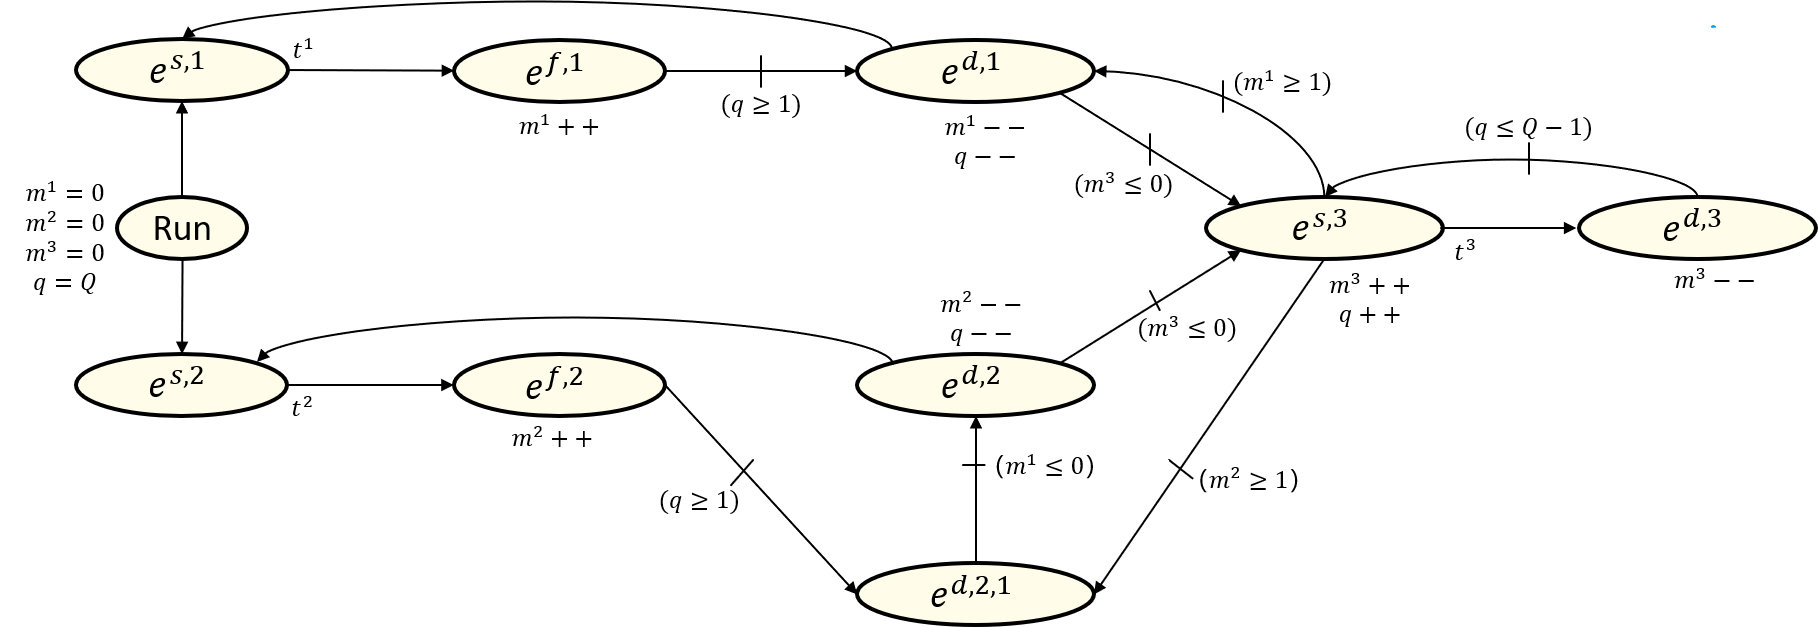
\includegraphics[width=0.7\textwidth]{Figures/ERG_merge.png}
	\caption{ERG of merge queueing system.}
	\label{fig:ERG_merge}
\end{figure}

It can be seen that the model proposed in \cite{chan2008optimization} requires to derive different constraints from each arcs according to the condition on the arc and to the state changes of several events. Furthermore, the constraints bound the event execution time from below, which indicates that the event \textit{can} be executed, and the objective function drives the events or each to be executed as soon as possible. However, the DES model \textit{must} execute the events once the conditions are true, which cannot be guaranteed with the model. To guarantee the equivalence between the MPR  and the simulation implementation, the multiplier of each term of the objective function has to be carefully chosen. Using the model proposed in this work, the objective function can be arbitrary, i.e., any performance indicator can be the objective function.


\section*{(s,S) policy}
\begin{table}[h]
	\begin{tabular}{lllllll} 
		\multicolumn{7}{l}{\textbf{Zero-delay events}}\\ \hline
		Variable&Event &  \multicolumn{4}{c}{Condition to schedule} & State change\\\hline
		$e^{\tilde{ca}}$ &Count customer arrival  &  \multicolumn{4}{c}{$u^{ca}\le 0$} & $u^{ca}${\footnotesize++} \\
		$e^{rr}$ & Require replenishment &  \multicolumn{4}{c}{$u^{ra}\le 0\ \&\ q\le s $} & $u^{ra}${\footnotesize++} \\
		$e^{cl}$ & Customer loss &  \multicolumn{4}{c}{$a\ge 1\ \&\ q\le0 $} & $a${\small-}{\small-}\\
		$e^{co}$ & Customer with order &  \multicolumn{4}{c}{$a\ge 1\ \&\ q\ge1 $} & $a${\small-}{\small-}, $q${\small-}{\small-} \\
		\multicolumn{7}{l}{\textbf{Positive-delay events}}\\ \hline
		Variable&Event 		   & Delay& $e^{\tilde{\xi}}$& $u^{\xi}$ &$\beta^{\xi}$& State change\\\hline
		$e^{ca}$&Customer order arrival & $T^{ca}$& $e^{\tilde{ca}}$&  $u^{ca}$&1&  $u^{ca}${\small-}{\small-}, $a${\footnotesize++}\\	
		$e^{ra}$&Replenishment arrival & $T^{ra}$& $e^{rr}$&  $u^{ra}$&1&  $u^{ra}${\small-}{\small-}, $q=q+S-s$\\	
		\hline
	\end{tabular}
	\caption{Events to simulate (s,S) policy.}
	\label{tab:sSpolicy}
\end{table}





\newpage
\newpage



\section{Draft}

\subsection{Condition based maintenance}

State variables
$b$: number of backorders
$q$: finished goods in queue
$m$: machine working/idle
$fl\in\{0,1,2\}$: failure level 
$r1$: first level repair
$r2$: second level repair

Events


\begin{table}[h]
	\begin{tabular}{lllllllll} 
		\multicolumn{9}{l}{\textbf{Zero-delay events}}\\ \hline
		Variable&Event &  \multicolumn{4}{c}{Condition to schedule} & State change&$N^{\xi}$&\\\hline
		$e^{\tilde{arr}}$ & Count arrival &  \multicolumn{4}{c}{$u^{arr}\le 0$} & $u^{arr}${\footnotesize++}&$N^1+N^2$& \\
		$e^{ol}$ & Order leaves&  \multicolumn{4}{c}{$b\ge 1,\ q\ge 1$} & $b${\small-}{\small-}, $q${\small-}{\small-}&$N^1$& \\
		$e^{oa}$ & Abandoned & \multicolumn{4}{c}{$b\ge B,\ so\ge 1$} &  $so${\small-}{\small-}&$N^2-B$&\\
		$e^{oe}$ & Order enters & \multicolumn{4}{c}{$b\le B-1,\ so\ge 1$} &  $so${\small-}{\small-}, $b${\footnotesize++}&$N^1+B$&\\
		$e^{s1}$ & Start & \multicolumn{4}{c}{$q\le Q-1,\ m\le 0,\  fl\le 1$} &  $m${\footnotesize++}&$??$&\\
		&& \multicolumn{4}{c}{$r1\le 0,\ (fl\le 0\ or\ q\le Q^r-1)$} &  &&\\
		$e^{sr1}$ & Start repair 1 & \multicolumn{4}{c}{$q\ge Q^r,\ m\le 0$} &  $r1${\footnotesize++}&$N^4$&\\	
		&& \multicolumn{4}{c}{$1\le fl\le 1,\ r1\le 0$} &  &&\\	
		$e^{sr2}$ & Start repair 2 & \multicolumn{4}{c}{$fl\ge 2,\ r2\le 0$} &  $r2${\footnotesize++}&$N^3-N^4$&\\	
		$e^{\tilde{fl1}}$ & Count failure 1 & \multicolumn{4}{c}{$fl\le 0,\ u^{fl1}\le 0$} & $u^{fl1}${\footnotesize++} &$N^3$&\\	
		$e^{\tilde{fl2}}$ & Count failure 2 & \multicolumn{4}{c}{$1\le fl\le 1,\ u^{fl2}\le 0$} & $u^{fl2}${\footnotesize++} &$N^3$&\\	
		&& \multicolumn{4}{c}{$r1\le 0$} &&&\\	
		\multicolumn{9}{l}{\textbf{Positive-delay events}}\\\hline
		Variable&Event 		   & Delay& $e^{\tilde{\xi}}$& $u^{\xi}$ &$\beta^{\xi}$& State change&$N^{\xi}$&Condition \\
		&&&&&&&&to cancel\\\hline
		$e^{arr}$&Arrival & $T^{arr}$& $e^{\tilde{arr}}$&  $u^{arr}$&1&  $u^{arr}${\small-}{\small-},  $so${\footnotesize++}&$N^1+N^2$&\\
		$e^{f}$&Finish & $T^{f}$& $e^{s}$&  $m$&1&  $m${\small-}{\small-},  $q${\footnotesize++}, $c^q${\footnotesize++}&$??$&$u^{fl2}\ge 1, m\ge 1$\\	
		$e^{fr1}$&Finish repair 1 & $T^{fr1}$& $e^{sr1}$&  $r1$&1& $fl${\small-}{\small-}, $r1${\small-}{\small-} &$N^4$&\\
		$e^{fr2}$&Finish repair 2 & $T^{fr2}$& $e^{sr2}$&  $r2$&1& $fl=fl-2$, $r2${\small-}{\small-}  &$N^3-N^4$&\\
		$e^{fl1}$&Failure 1 & $T^{fl1}$& $e^{\tilde{fl1}}$&  $u^{fl1}$&1& $fl${\footnotesize++}, $u^{fl1}${\small-}{\small-} &$N^3$&\\
		$e^{fl2}$&Failure 2 & $T^{fl2}$& $e^{\tilde{fl2}}$&  $u^{fl2}$&1& $fl${\footnotesize++}, $u^{fl2}${\small-}{\small-}  &$N^3$&$r1\ge 1$, $u^{fl2}\ge 1$\\	
		\hline
	\end{tabular}
	\caption{Events to simulate G/G/1 with failure.}
	\label{tab:maintenance}
\end{table}







MP model of single server merge model:
\begin{eqnarray}
\min{\sum_{k}\mathcal{E}_k}\\
e^{(\xi,j),1}_i - \mathcal{E}_{k}\ge M(w^{\xi,j}_{i,k}-1)&&\xi\in\{s,f,d\}, j\in\{1,2,3\},\forall i,k \\
\mathcal{E}_{k} - e^{(\xi,j),1}_i\ge M(w^{\xi,j}_{i,k}-1)&&\xi\in\{s,f,d\}, j\in\{1,2,3\},\forall i,k \\
\sum_{k} w^{\xi,j}_{i,k} =1&& \forall\ \xi\in\{s,f,d\}, j\in\{1,2,3\},i\\
\sum_{(\xi,j),i} w^{\xi,j}_{i,k} =1&& \forall\ k\\
\sum_{k} kw^{\xi,j}_{i+1,k} - \sum_{k} kw^{\xi,j}_{i,k} \ge 1&& \forall\  \xi\in\{s,f,d\}, j\in\{1,2,3\},i\\
e^{s,j,1}_{i} - e^{s,j,0}_{i} \ge 0 && j =1,2,3, \forall \ i\\
e^{f,j,1}_{i} - e^{f,j,0}_{i} \ge t^j_{i}&& j =1,2, \forall \ i\\
e^{d,j,1}_{i} - e^{d,j,0}_{i} \ge 0 && j =1,2, \forall \ i\\
e^{d,3,1}_{i} - e^{d,3,0}_{i} \ge t^3_{i}&&\forall \ i \\
e^{\xi,j,0}_i-\mathcal{E}_{k} \ge M(x^{\xi,j}_{i,k}-1)&& \forall\ \xi\in\{s,f,d\},j=1,2,3,k,i\\
\mathcal{E}_{k} -e^{\xi,j,0}_i\ge M(x^{\xi,j}_{i,k}-1)&& \forall\ \xi\in\{s,f,d\},j=1,2,3,k,i\\
m^j_k=m^j_{k-1} + \sum_{i=1}^{N^{j}} (w^{s,j}_{i,k}  + w^{f,j}_{i,k} - 2w^{d,j}_{i,k})&& j=1,2, \forall\ k\\
m^3_k=m^3_{k-1} + \sum_{i=1}^{N^{3}} (w^{s,3}_{i,k} - w^{d,3}_{i,k})&&\forall\ k\\
q_k = q_{k-1} + \sum_{i=1}^{N^{3}} w^{s,3}_{i,k} - \sum_{i=1}^{N^{1}} w^{d,1}_{i,k} - \sum_{i=1}^{N^{2}} w^{d,2}_{i,k}\\
m^j_k \ge M(z^{s,j}_{k}-1)&& j=1,2,3, \forall \ k\\
1- m^j_k \ge M(z^{f,j}_{k}-1)&& j=1,2, \forall \ k\\
m^j_k - 1 \ge M(z^{f,j}_{k}-1)&& j=1,2, \forall \ k\\
m^j_k - 2 \ge M(z^{d,j}_{k}-1)&& j=1,2, \forall \ k\\
q_k - 1 \ge M(z^{d,j}_{k}-1)&&  j=1,2, \forall \ k\\
1 - m^1_k \ge M(z^{d,2}_{k}-1)&& \forall\ k\\
m^3_k - 1 \ge M(z^{d,3}_{k}-1)&& \forall \ k\\
(Q-1) - q_k \ge M(z^{s,3}_{k}-1)&& \forall\ k\\
\sum_{k} x^{\xi,j}_{i,k} =1&& \forall\ \xi\in\{s,f,d\}, j=1,2,3, \forall\ i,k\\
\sum_{i=1}^{N^{j}}x^{\xi,j}_{i,k} \le z^{\xi,j}_{k}&& \forall\ \xi\in\{s,f,d\}, j=1,2,3, k\\
\sum_{k} kx^{\xi,j}_{i+1,k} - \sum_{k} kx^{\xi,j}_{i,k} \ge 0 && \forall\ \xi\in\{s,f,d\}, j=1,2,3, i
\end{eqnarray}


\section{Resource allocation problem of queueing systems}
\subsection{Mathematical programming representation of simulation model}
We study only the system that the occurrence of an event will lead to the increment or decrement of one unit of the state variables. A simulation model is called a \textit{natural} simulator if the following assumptions all hold:
\begin{enumerate}
		\item An event $e^{\xi}$ can be triggered if the state variables $\mathbf{s}$ satisfy specific conditions \textit{at that time}, regardless of the history of the state or event occurrence, and the condition is not changed along time, i.e., condition is static. It could be possible to define more state variables in case of history dependence and variant triggering conditions.
		\item Natural triggering relationship: if and only if $e^{\xi}$ is an $s$-increment event, $e^{\xi}$ triggers an $s$-decrement event, vice versa.
		\item Natural triggering condition: the condition for triggering an $e^{\xi}$ is that each state variable $s$ must within its predefined domain, i.e., $\mathbf{l} \le\mathbf{s}\le \mathbf{u}$, regardless of event type $\xi$.
		\item For all $e^{\xi}$, the number of execution $N^{\xi}$ is known before simulation, and the simulation terminate when all types of events have been triggered for that number.
\end{enumerate}

Assumptions for a variable $x$ to be resource-type:
\begin{enumerate}
	\item For all $e^{\xi}$, $\mathbf{u}$ is monotonically increasing on $x$, and $\mathbf{l}$ is monotonically decreasing on $x$.
	%\item The condition for triggering an $e^{\xi}$ is in the form of \textit{range}, i.e., $\mathbf{l}^{\xi} \le\mathbf{s}\le \mathbf^{u}^{\xi}$.
	%\item For all $e^{\xi}$, $\mathbf^{u}^{\xi}$ is monotonically increasing on $x$, and $\mathbf{l}^{\xi}$ is monotonically decreasing on $x$.
\end{enumerate}

Formulate the MP model of simulation:

\begin{table}[h]
	\begin{tabular}{ll}
		\hline
		$e^{\xi}_{i}\ge 0$ & time of the $i$-th occurrence of event $e^{\xi}$.\\
		$\tau^{s+}_{l}\ge 0$ & time of the  $l$-th occurrence of events that increments state variable $s$.\\
		$\tau^{s-}_{l}\ge 0$ &   time of the  $l$-th occurrence of events that decrements state variable $s.$\\
		%$c^{\xi,s}_{l}$& the occurring time $l$-th candidate event to trigger event $e^{\xi}$  respect to the condition of state variable $s$.\\		
		$x^{\xi,s+}_{i,l}\in\{0,1\}$& equal to 1 if $e^{\xi}_{i}$ is the $l$-th increment of $s$.\\
		$x^{\xi,s-}_{i,l}\in\{0,1\}$& equal to 1 if $e^{\xi}_{i}$ is the $l$-th decrement of $s$.\\\hline
		%$y^{\xi,s}_{i,l}\in\{0,1\}$ & equal to 1 if the $l$-th candidate event $c^{\xi,s}_{l}$ triggers $e^{\xi}_{i}$.
	\end{tabular}
\end{table} 


The MP model of simulation is
\begin{eqnarray}
&\min\{\sum_{\xi,i} e^{\xi}_{i}\}&\\
&s.t.&\\
&\tau^{s+}_{l} - \tau^{s-}_{l+s_0-u_s} \ge 0& \forall\ s \\
&\tau^{s-}_{l} - \tau^{s+}_{l-s_0+l_s} \ge 0& \forall\ s \\
&\tau^{s+}_{l} - e^{\xi}_{i} \ge M(x^{\xi,s+}_{i,l}-1)& \forall\ s\ and\ e^{\xi}\ with\ increment\ of\ s\\
&\tau^{s-}_{l} - e^{\xi}_{i} \ge M(x^{\xi,s-}_{i,l}-1)& \forall\ s\ and\ e^{\xi}\ with\ decrement\ of\ s\\
&e^{\xi}_{i} - \tau^{s+}_{l} \ge M(x^{\xi,s+}_{i,l}-1) & \forall\ s\ and\ e^{\xi}\ with\ increment\ of\ s\\
&e^{\xi}_{i} - \tau^{s-}_{l} \ge M(x^{\xi,s-}_{i,l}-1) & \forall\ s\ and\ e^{\xi}\ with\ decrement\ of\ s\\
&\sum_{\xi,i} x^{\xi,s+}_{i,l} =1& \forall\ s,l\\
&\sum_{\xi,i} x^{\xi,s-}_{i,l} =1& \forall\ s,l\\
&\sum_{s,l} x^{\xi,s+}_{i,l} =1& \forall\ \xi,i\\
&\sum_{s,l} x^{\xi,s-}_{i,l} =1& \forall\ \xi,i\\
\end{eqnarray}


\newpage
\subsection{Mathematical programming representation of simulation model - V2}

Revise event-based simulation algorithm.

\begin{figure}[h]
	\centering
	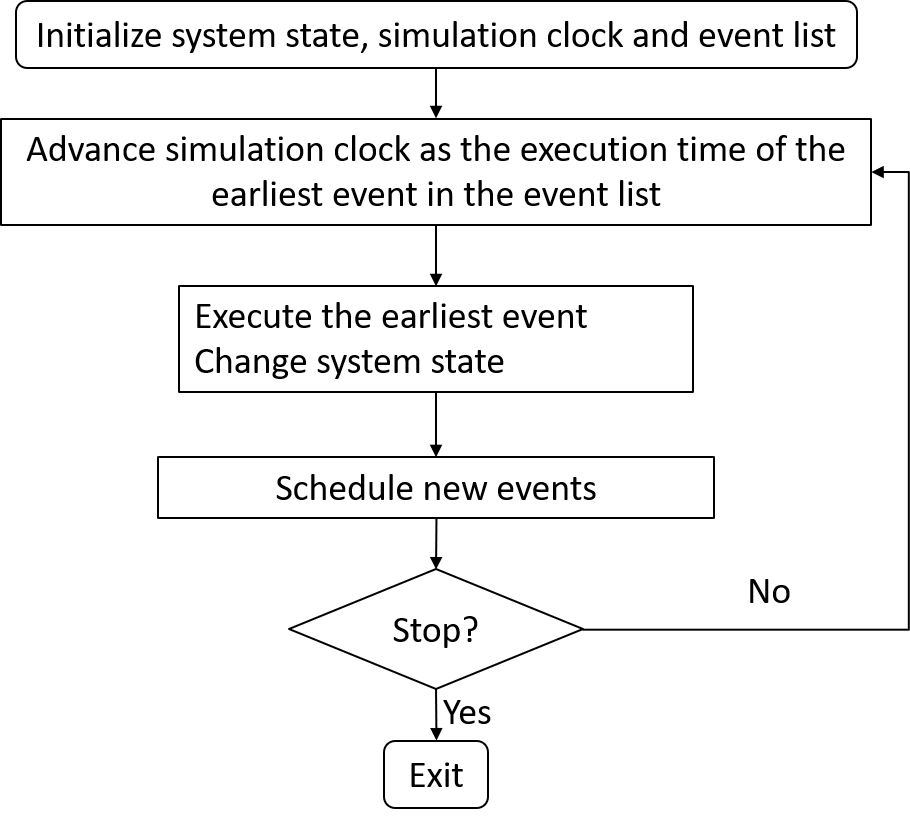
\includegraphics[width=0.6\textwidth]{Figures/EventSimAlgo.png}
	\caption{Event-based simulation algorithm.}
	\label{fig:EventSimAlgo}
\end{figure}

An equivalent mathematical programming model exists if the following assumptions are satisfied:
\begin{enumerate}
	\item State variables are integer.
	\item For all event $e^{\xi}$, the \textit{scheduling conditions} are in the form of $a^{\xi}_s\le s \le c^{\xi}_s$ combined with logic operator ``AND", where $s$ is a state variable, and $a^{\xi}_s$ and $c^{\xi}_s$ are lower and upper bounds.
	\item The scheduling conditions is independent of the history and not changed along time. (It could be possible to define more state variables in case of history dependence and time-variant scheduling conditions.)
	\item An event execution of $e^{\xi}$ leads to integer increment or decrement equal to $\Delta^{\xi}_s$ of certain state variables $s$, and $\Delta^{\xi}_s$ is not changed along time.
	\item The delay between scheduling and execution time of an event $e^{\xi}$, denoted by $t^{\xi}$, is random variate. They can be generated independently from the simulation run. (\textit{This point is different from ERG. In ERG, the delay is dependent on the edge, i.e, a couple of events, but I consider delay dependent on a single event.})
	\item For all events $e^{\xi}$, the number of executions $\mathbb{I}^{\xi}$ is known before simulation.
\end{enumerate}

\begin{table}[h]
	\begin{tabular}{ll}
		$e^{\xi}$ & event of type $\xi$\\
		$s$& state variable\\
		$\mathbb{S}$& set of all state variables\\
		$\mathbb{S}^{\xi}$  & set of state variables whose value is conditioned for scheduling event $e^{\xi}$.\\
		$\Theta^{\xi+}$ & the set of state variables that event $e^{\xi}$ will increase its value.\\
		$\Theta^{\xi-}$ & the set of state variables that event $e^{\xi}$ will decrease its value.\\
		$\Theta^{\xi}$ & $\Theta^{\xi+}\cap\Theta^{\xi-}$\\
		$E^{s+}$ & set of events whose execution increases the value of state variable $s$.\\
		$E^{s-}$  & set of events whose execution decreases the value of state variable $s$.\\
		$\Delta^{\xi}_s$ & increment or decrement of state variable $s$ when event $e^{\xi}$ is executed.\\
		$I^{\xi}$ & total number of executions of event $e^{\xi}$\\
		$L^{s+}$& total number of  times that state variable $s$ is increased.\\
		$L^{s-}$ & total number of  times that state variable $s$ is decreased.\\
		$t^{\xi}$ & delay between scheduling and execution of event $e^{\xi}$.\\
		$t^{\xi}_i$ & delay between $i$-th scheduling and its execution of event $e^{\xi}$.\\
	\end{tabular}
\caption{Notations}
\end{table}


\textbf{Preparation} Event $e^{\xi}$ is expanded into a series of events $e^{\xi,0}$, $e^{\xi,1}$, ..., $e^{\xi,\Delta^{\xi}}$, where $\Delta^{\xi}$ is equal to the maximum among $\Delta^{\xi}_s$ for all $s\in \Theta^{\xi}$. The expansion is conducted as follows. First, event $e^{\xi,0}$ is executed as soon as all the scheduling conditions are satisfied, and the state variables $s\in \Theta^{\xi}$ are not changed. Then, event $e^{\xi,1}$ is executed after $t^{\xi}$ time unit after an execution of $e^{\xi,0}$. For all $s\in \Theta^{\xi}$, if $\Delta^{\xi}_s\ge \delta$,  $e^{\xi,\delta}$ will increase or decrease $s$ by one, for all $\delta=1,...,\Delta^{\xi}$. The $i$-th execution of event $e^{\xi,\delta}$ for $\delta=1,...,\Delta^{\xi}$ are simultaneous.



\begin{table}[h]
	\begin{tabular}{ll}
		$e^{\xi,\delta}_i\ge 0$ 	& time of $i$-th execution of event $e^{\xi,\delta}$\\
		$\tau^{s+}_{l}\ge 0$ 			& time when state variable $s$ is increased for the $l$-th time.  \\
		$\tau^{s-}_{l}\ge 0$ 			& time when state variable $s$ is decreased for the $l$-th time. \\
		$x^{\xi}_{i,i^{'}}\in \{0,1\}$ 	& equal to 1 if the $i^{'}$ execution of event $e^{\xi}$ is the $i$-th scheduled one. \\
		$y^{\xi,\delta,s+}_{i,l}\in \{0,1\}$ & equal to 1 if the $i$-th execution of event $e^{\xi}$ is the $l$-th time that state variable $s$ in increased.\\
		$y^{\xi,\delta,s-}_{i,l}\in \{0,1\}$ &equal to 1 if the $i$-th execution of event $e^{\xi}$ is the $l$-th time that state variable $s$ in decreased.\\
		$z^{\xi,s+}_{i,l}\in \{0,1\}$ & equal to 1 if the $i$-th scheduling of event $e^{\xi}$ is later than $\tau^{s+}_{l}$.\\
	\end{tabular}
\caption{Decision variables}
\end{table}


\textbf{Constraints (A)} The constraints below imply that event $e^{\xi,1}$ is scheduled to execute with a delay $t^{\xi}$, after an execution of $e^{\xi,0}$. 
\begin{eqnarray}
e^{\xi,1}_{i^{'}} - e^{\xi,0}_{i} \ge t^{\xi}_{i} +M(x^{\xi}_{i,i^{'}}-1) && \forall \xi, i, i ^{'}=1,...,I^{\xi}\label{eq::A1}
\end{eqnarray}

It should be noticed that, if multiple executions of the same event $e^{\xi}$ are allow to exist in the future event list simultaneously, the execution of $e^{\xi,1}$ scheduled by the $i$-th execution of $e^{\xi,0}$ may be not the $i$-th execution of $e^{\xi,1}$. Thus, binary variables $x^{\xi}_{i,i^{'}}$ are introduced, and it is equal to one if the $i^{'}$ execution of event $e^{\xi,1}$ is scheduled by the $i$-th execution of event $e^{\xi,0}$. Since each execution of $e^{\xi,0}$ can schedule one and only one execution of $e^{\xi,1}$, the following constraints should also be satisfied:
\begin{eqnarray}
\sum_{i=1}^{N^{\xi}} x^{\xi}_{i,i^{'}} = 1&& \forall\ \xi, i^{'}=1,...,I^{\xi}\\
\sum_{i^{'}=1}^{N^{\xi}} x^{\xi}_{i,i^{'}} = 1 && \forall\ \xi,i=1,...,I^{\xi}
\end{eqnarray}

If up to $\alpha^{\xi}$ multiple executions of event $e^{\xi}$ are allowed, the following constraints can be added:

\begin{eqnarray}
e^{\xi,0}_{i} - e^{\xi,1}_{i-\alpha^{\xi}} \ge 0 && \forall\ \xi,\ i=\alpha^{\xi}+1,...,I^{\xi} \\
\sum_{i^{'}=i+\alpha^{\xi}}^{I^{\xi}} x^{\xi}_{i,i^{'}}=0&& \forall\ \xi,\ i=1,...,I^{\xi}-\alpha^{\xi}\\
\sum_{i=1}^{i^{'}-\alpha^{\xi}} x^{\xi}_{i,i^{'}}=0&&\forall\ \xi,\ i^{'}=\alpha^{\xi}+1, ..., I^{\xi}
\end{eqnarray}

If $\alpha^{\xi}$ is equal to one, the constraints (A) are reduced to:
\begin{eqnarray}
e^{\xi,1}_{i} - e^{\xi,0}_{i} \ge t^{\xi}_{i} && \forall \xi, i=1,...,I^{\xi}\\
e^{\xi,0}_{i} - e^{\xi,1}_{i-1} \ge 0&& \forall\ \xi,\ i=2,...,I^{\xi} 
\end{eqnarray}

\textbf{Constraints (B)} Binding $e^{\xi,\delta}_i$ and $\tau^{s+}_l,\ \tau^{s-}_l$:
\begin{eqnarray}
\tau^{s+}_l - e^{\xi,\delta}_i \ge M(y^{\xi,\delta,s+}_{i,l}-1)&&\forall\ s\in \mathbb{S},e^{\xi}\in E^{s+},\delta=1,..,\Delta^{\xi}_s,i=1,..,I^{\xi},l=1,..,L^{s+} \\
e^{\xi,\delta}_i - \tau^{s+}_l \ge M(y^{\xi,\delta,s+}_{i,l}-1)&&\forall\ s\in \mathbb{S},e^{\xi}\in E^{s+},\delta=1,..,\Delta^{\xi}_s,i=1,..,I^{\xi},l=1,..,L^{s+}\\
\tau^{s-}_l - e^{\xi,\delta}_i \ge M(y^{\xi,\delta,s-}_{i,l}-1)&&\forall\ s\in \mathbb{S},e^{\xi}\in E^{s-},\delta=1,..,\Delta^{\xi}_s,i=1,..,I^{\xi},l=1,..,L^{s-}\\
e^{\xi,\delta}_i - \tau^{s-}_l \ge M(y^{\xi,\delta,s-}_{i,l}-1)&&\forall\ s\in \mathbb{S},e^{\xi}\in E^{s-},\delta=1,..,\Delta^{\xi}_s,i=1,..,I^{\xi},l=1,..,L^{s-}\\
\sum_{\begin{subarray}{c} \xi:e^{\xi}\in E^{s+} \\ i=1,...,I^{\xi}\\\Delta=1,..., \Delta^{\xi}_s\end{subarray}} y^{\xi,\delta,s+}_{i,l}=1&& \forall\ s\in \mathbb{S},l=1,...,L^{s+}\\
\sum_{l=1,...,L^{s+}} y^{\xi,\delta,s+}_{i,l}=1&&\forall\ \xi,s\in \Theta^{\xi+},i=1,...,I^{\xi},\delta=1,...,\Delta^{\xi}_{s}\\
\sum_{\begin{subarray}{c} \xi:e^{\xi}\in E^{s-} \\ i=1,...,I^{\xi}\\\Delta=1,..., \Delta^{\xi}_s\end{subarray}} y^{\xi,\delta,s-}_{i,l}=1&& \forall\ s\in \mathbb{S},l=1,...,L^{s-}\\
\sum_{l=1,...,L^{s-}} y^{\xi,\delta,s-}_{i,l}=1&&\forall\ \xi, s\in \Theta^{\xi-}, i=1,...,I^{\xi},\delta=1,...,\Delta^{\xi}_{s}\\
\end{eqnarray}

Binary variables $y^{\xi,\delta,s+}_{i,l}\in \{0,1\}$ are equal to one if the $i$-th execution of event $e^{\xi,\delta}$ is the $l$-th time that state variable $s$ in increased. Since events $e^{\xi,1},...,e^{\xi,\Delta^{\xi}_s}$ are expanded from one event $e^{\xi}$, and they are executed simultaneously, the following constraints are also added:
\begin{eqnarray}
e^{\xi,\delta}_i = e^{\xi,1}_i && \forall\ \xi,\ i=1,...,I^{\xi}, \delta=1,...,\Delta^{\xi}\\
y^{\xi,\delta,s+}_{i,l+\delta-1} = y^{\xi,1,s+}_{i,l} &&\forall\ \xi,\ s\in\Theta^{\xi+},\ \delta=1,...,\Delta^{\xi}_s,\ i=1,...,I^{\xi}, \ l=1,...,L^{s+}-\Delta^{\xi}_s+1\\
y^{\xi,\delta,s-}_{i,l+\delta-1} = y^{\xi,1,s-}_{i,l} &&\forall\ \xi,\ s\in\Theta^{\xi-},\ \delta=1,...,\Delta^{\xi}_s,\ i=1,...,I^{\xi}, \ l=1,...,L^{s-}-\Delta^{\xi}_s+1
\end{eqnarray}


\textbf{Constraints (C)} To trigger event $e^{\xi,0}$, the conditions $b^{\xi}_s\le s\le c^{\xi}_s$ for all state variable $s\in \mathbb{S}^{\xi}$ should be satisfied. $s\in \mathbb{S}^{\xi}$ can be categorized into one of the following three situations:
\begin{itemize}
	\item event $e^{\xi}$ does not change the value of $s$, i.e., $s\notin \Theta^{\xi}$.
	\item event $e^{\xi}$ increases the value of $s$, i.e., $s\in \Theta^{\xi+}$. 
	\item event $e^{\xi}$ decreases the value of $s$, i.e., $s\in \Theta^{\xi-}$. 
\end{itemize}

If event $e^{\xi}$ does not change the value of $s$, or if it is executed after being scheduled with positive delay, i.e., $s\notin \Theta^{\xi}$ or $t^{\xi}>0$, the following constraints are applied:
\begin{eqnarray}
e^{\xi,0}_{i} - \tau_{l}^{s+} \le Mz^{\xi,s+}_{i,l} & \forall\ \xi,i=1,...,I^{\xi},\ s\in \mathbb{S}^{\xi}, l=1,....,L^{s+}\\
e^{\xi,0}_{i} - \tau_{l}^{s-} \le Mz^{\xi,s-}_{i,l} & \forall\ \xi,\ i=1,...,I^{\xi},\ s\in \mathbb{S}^{\xi}, l=1,....,L^{s-}\\
e^{\xi,0}_{i} - \tau_{l}^{s-} \ge -M\hat{z}^{\xi,s-}_{i,l}& \forall\ \xi,\ i=1,...,I^{\xi},\ s\in \mathbb{S}^{\xi}, l=1,....,L^{s-}\\
e^{\xi,0}_{i} - \tau_{l}^{s+} \ge -M\hat{z}^{\xi,s+}_{i,l}& \forall\ \xi,\ i=1,...,I^{\xi},\ s\in \mathbb{S}^{\xi}, l=1,....,L^{s+}\\
%e^{\xi,0}_{i} - \tau_{s_0+l-b^{\xi}_{s}}^{s-} \ge -M\hat{z}^{\xi,s-}_{i,l}& \forall\ \xi,\ i=1,...,I^{\xi},\ s\in \mathbb{S}^{\xi}, l=1,....,L^{s-}??\\
%e^{\xi,0}_{i} - \tau_{-s_0+l+a^{\xi}_{s}}^{s+} \ge -M\hat{z}^{\xi,s+}_{i,l}& \forall\ \xi,\ i=1,...,I^{\xi},\ s\in \mathbb{S}^{\xi}, l=1,....,L^{s+}??\\
z^{\xi,s+}_{i,l}+\hat{z}^{\xi,s-}_{i,s_0+l-b^{\xi}_{s}}\le 1&??\\
z^{\xi,s-}_{i,l}+\hat{z}^{\xi,s+}_{i,-s_0+l+a^{\xi}_{s}}\le 1&??\\
%z^{\xi,s+}_{i,l}+\hat{z}^{\xi,s-}_{i,l}\le 1&??\\
%z^{\xi,s-}_{i,l}+\hat{z}^{\xi,s+}_{i,l}\le 1&??
\end{eqnarray}

\begin{eqnarray}
e^{\xi,0}_{i} - \tau_{l}^{s+} \ge M(z^{\xi,s+}_{i,l}-1) & \forall\ \xi,i=1,...,I^{\xi},\ s\in \mathbb{S}^{\xi}, l=1,....,L^{s+}\\
\tau_{l}^{s+} - e^{\xi,0}_{i} > -Mz^{\xi,s+}_{i,l}& \forall\ \xi,\ i=1,...,I^{\xi},\ s\in \mathbb{S}^{\xi}, l=1,....,L^{s+}\\
e^{\xi,0}_{i} - \tau_{l}^{s-} \ge M(z^{\xi,s-}_{i,l}-1) & \forall\ \xi,\ i=1,...,I^{\xi},\ s\in \mathbb{S}^{\xi}, l=1,....,L^{s-}\\
\tau_{l}^{s-} - e^{\xi,0}_{i} > -Mz^{\xi,s-}_{i,l}& \forall\ \xi,\ i=1,...,I^{\xi},\ s\in \mathbb{S}^{\xi}, l=1,....,L^{s-}\\
\end{eqnarray}







If $e^{\xi,0}_{i}$ is executed after $\tau_{l}^{s+}$($\tau_{l}^{s-}$), $z^{\xi,s+}_{i,l}$($z^{\xi,s-}_{i,l}$) is equal to one. If $e^{\xi,0}_{i}$ is executed before $\tau_{l}^{s+}$($\tau_{l}^{s-}$), $\hat{z}^{\xi,s+}_{i,l}$($\hat{z}^{\xi,s-}_{i,l}$) is equal to one.


If event $e^{\xi}$ increases the value of $s$, and it is executed immediately when scheduled, i.e., $s\in \Theta^{\xi+}$ and $t^{\xi}=0$, the following constraint should be applied:
\begin{eqnarray}
e^{\xi,0} - \tau^{s-}_{s_0+l-1-b} \ge M(y^{\xi,1,s+}_{i,l}-1)\\
e^{\xi,0} - \tau^{s-}_{s_0+l-1-a} \le M(1-y^{\xi,1,s+}_{i,l})
\end{eqnarray}

If event $e^{\xi}$ decreases the value of $s$, and it is executed immediately when scheduled, i.e., $s\in \Theta^{\xi-}$ and $t^{\xi}=0$, the following constraint should be applied:
\begin{eqnarray}
e^{\xi,0} - \tau^{s+}_{-s_0+l-1+a} \ge M(y^{\xi,1,s-}_{i,l}-1)\\
e^{\xi,0} - \tau^{s+}_{-s_0+l-1+b} \le M(1-y^{\xi,1,s-}_{i,l})
\end{eqnarray}



\newpage
\subsection{Mathematical programming representation of simulation model - V3}
Event-scheduling algorithm for DES. 

\begin{figure}[h]
	\centering
	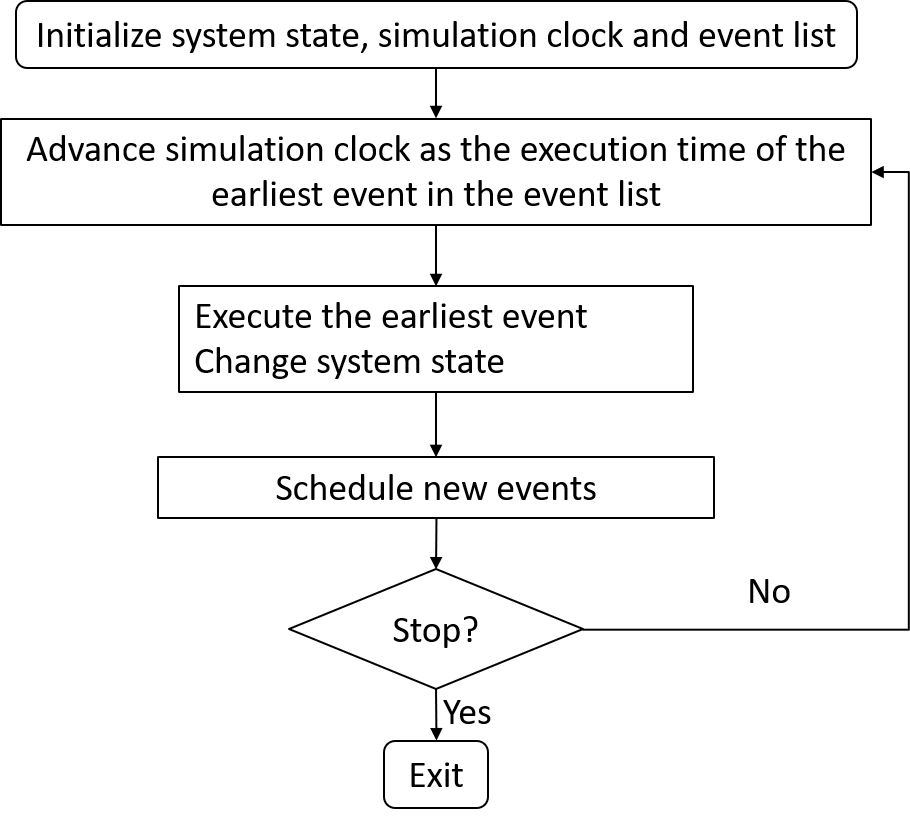
\includegraphics[width=0.8\textwidth]{Figures/EventSimAlgo.png}
	\caption{Event-based simulation algorithm.}
\end{figure}


An equivalent mathematical programming model exists if the following assumptions are satisfied:
\begin{enumerate}
	% \item State variables are integer.
	\item For all event $e^{\xi}$, the \textit{scheduling conditions} are in the form of $b^{\xi}_s\le s \le c^{\xi}_s$ combined with logic operator ``AND", where $s$ is a state variable, and $b^{\xi}_s$ and $c^{\xi}_s$ are lower and upper bounds.
	\item The scheduling conditions is independent of the history and not changed along time. (It could be possible to define more state variables in case of history dependence and time-variant scheduling conditions.)
	\item An event execution of $e^{\xi}$ leads to (integer) increment or decrement equal to $\Delta^{\xi}_s$ of certain state variables $s$, and $\Delta^{\xi}_s$ is not changed along time. (A direct evaluation can be modeled in this way.)
	\item The delay between scheduling and execution time of an event $e^{\xi}$, denoted by $t^{\xi}$, is random variate. They can be generated independently from the simulation run. (\textit{This point is different from ERG. In ERG, the delay is dependent on the edge, i.e, a couple of events, but I consider delay dependent on a single event.})
	\item For all events $e^{\xi}$, the number of executions $N^{\xi}$ is known before simulation.
\end{enumerate}

\begin{table}[h]
	\begin{tabular}{lll}
		$e^{\xi,0}_{i}\ge 0$ & $i$=1,...,$I^{\xi}$& the $i$-th scheduling time of event $e^{\xi}$.\\
		$e^{\xi,1}_{i}\ge 0$ & $i$=1,...,$I^{\xi}$& the $i$-th execution time of event $e^{\xi}$.\\
		$\mathcal{E}_k\ge 0$ &$k$=0,...,$\mathbb{K}$& time of the $k$-th execution of any events.\\
		$u^s_k\in \mathbb{Z}$ &$k$=0,...,$\mathbb{K}$& value of state variable $s$ just after the $k$-th event.\\
		$w^{\xi}_{i,k}\in \{0,1\}$ &$k$=1,...,$\mathbb{K}$& binding $e^{\xi,1}_i$ and $\mathcal{E}_k$.\\
		$x^{\xi}_{i,k}\in\{0,1\}$ &$k$=0,...,$\mathbb{K}$& equal to one if $\mathcal{E}_k$ schedules $e^{\xi,0}$.\\
		$y^{\xi}_{i,i^{'}}\in\{0,1\}$&& binding $e^{\xi,0}_i$ and $e^{\xi,1}_{i^{'}}$ in case of overtaking.\\
		$z^{\xi}_{k}\in\{0,1\}$ &$k$=0,...,$\mathbb{K}$& equal to one if the condition for scheduling $e^{\xi}$ is true right after $\mathcal{E}_k$.\\ 
		$v^{\xi,s,0}_k\in\{0,1\}$ &$k$=0,...,$\mathbb{K}$& equal to one if $s_k\le a^{\xi,s}-1$\\
		$v^{\xi,s,1}_k\in\{0,1\}$ &$k$=0,...,$\mathbb{K}$& equal to one if $s_k\ge b^{\xi,s}-1$\\
		$r^{\xi}_k\in \mathbb{Z}$ &$k$=0,...,$\mathbb{K}$& number of existing parallel executions of $e^{\xi,1}_i$ after $\mathcal{E}_k$ before scheduling.\\
		$n^{\xi}_k\in \mathbb{Z}$ & $k$=0,...,$\mathbb{K}$ & number of scheduled executions of $e^{\xi,1}_i$ after $\mathcal{E}_k$ before scheduling.\\
	\end{tabular}
\caption{Notation}
\end{table}

\textbf{Constraints (A):} binding $e^{\xi,1}_i$ and $\mathcal{E}_k$:
\begin{eqnarray}
	e^{\xi,1}_i-\mathcal{E}_k\ge M(w^{\xi}_{i,k}-1) &A1& \forall\ \xi,i,k\\
	\mathcal{E}_k-e^{\xi,1}_i\ge M(w^{\xi}_{i,k}-1) &A2& \forall\ \xi,i,k\\
	\sum_{k} w^{\xi}_{i,k} =1&A3& \forall\ \xi,i\\
	\sum_{\xi,i} w^{\xi}_{i,k} =1&A4& \forall\ k\\
	\sum_{k} kw^{\xi}_{i+1,k} - \sum_{k} kw^{\xi}_{i,k} \ge 1&A5& \forall\ \xi,i
\end{eqnarray}

\textbf{Constraints (B):} binding $e^{\xi,0}_i$ and $e^{\xi,1}_{i^{'}}$, where $\alpha^{\xi}$ is the maximal number of executions existing simultaneously in the event list:
\begin{eqnarray}
e^{\xi,1}_{i^{'}} - e^{\xi,0}_{i} \ge t^{\xi}_{i} +M(y^{\xi}_{i,i^{'}}-1) &B1& \forall \xi, i, i ^{'}=1,...,N^{\xi}\\
e^{\xi,0}_{i} - e^{\xi,1}_{i^{'}}  \ge -t^{\xi}_{i} +M(y^{\xi}_{i,i^{'}}-1) &B2& \forall \xi, i, i ^{'}=1,...,N^{\xi}\\
\sum_{i=1}^{N^{\xi}} y^{\xi}_{i,i^{'}} = 1&B3& \forall\ \xi, i^{'}=1,...,N^{\xi}\\
\sum_{i^{'}=1}^{N^{\xi}} y^{\xi}_{i,i^{'}} = 1 &B4& \forall\ \xi,i=1,...,N^{\xi}\\
%e^{\xi,0}_{i} - e^{\xi,1}_{i-\alpha^{\xi}} \ge 0 && \forall\ \xi,\ i=\alpha^{\xi}+1,...,N^{\xi} \\
\sum_{i^{'}=i+\alpha^{\xi}}^{N^{\xi}} y^{\xi}_{i,i^{'}}=0&B5& \forall\ \xi,\ i=1,...,N^{\xi}-\alpha^{\xi}\\
\sum_{i=1}^{i^{'}-\alpha^{\xi}} y^{\xi}_{i,i^{'}}=0&B6&\forall\ \xi,\ i^{'}=\alpha^{\xi}+1, ..., N^{\xi}
\end{eqnarray}
If $\alpha^{\xi}=1$, variables $y^{\xi}_{i,i^{'}}$ are redundant and constraints (B) are reduced to:
\begin{eqnarray}
e^{\xi,1}_{i} - e^{\xi,0}_{i} = t^{\xi}_{i} &B1& \forall \xi, i=1,...,N^{\xi}
% e^{\xi,0}_{i} - e^{\xi,1}_{i-1} \ge 0 && \forall\ \xi,\ i=2,...,N^{\xi} 
\end{eqnarray}
Number of executions of event $e^{\xi}$ waiting in the event list can be a state variable $n^{\xi}$, and one condition for scheduling an $e^{\xi}$ is $n^{\xi}\le \alpha^{\xi}$. Thus, it can be managed as a generic scheduling condition.

\textbf{Constraints (C):} event $e^{\xi}$ can be scheduled right after $\mathcal{E}_k$ if all state variables $s$ satisfies condition $a^{\xi}_{s}\le s_k\le b^{\xi}_{s}$. 
\begin{eqnarray}
e^{\xi,0}_i-\mathcal{E}_{k} \ge M(x^{\xi}_{i,k}-1)&C1& \forall\ \xi,k,i\\
\mathcal{E}_{k} -e^{\xi,0}_i\ge M(x^{\xi}_{i,k}-1)&C2& \forall\ \xi,k,i\\
\sum_{k} x^{\xi}_{i,k} =1&C3& \forall\ \xi,i\\
b^{\xi,s} - u^s_k \ge M(z^{\xi}_{k}-1)&C4& \forall\ \xi, k,s\\
% - u^s_k \ge U^{s}(z^{\xi}_{k}-1)-b^{\xi,s}z^{\xi}_{k}&C4& \forall\ \xi, k,s\\
 u^s_k - a^{\xi,s} \ge M(z^{\xi}_{k}-1)&C5& \forall\ \xi, k,s\\
%u^s_k  \ge a^{\xi,s}z^{\xi}_{k} -L^{s}(z^{\xi}_{k}-1)&C5& \forall\ \xi, k,s\\
u^s_k -  (b^{\xi,s}+1) \ge M(v^{\xi,s,1}_k-1) &C6& \forall\ \xi,k,s\\
%u^s_k \ge (b^{\xi,s}+1)v^{\xi,s,1}_k -L^s(v^{\xi,s,1}_k-1)&C6& \forall\ \xi,k,s\\
( a^{\xi,s}-1) - u^s_k \ge M(v^{\xi,s,0}_k-1) &C7& \forall\ \xi,k,s\\
% - u^s_k \ge U^s(v^{\xi,s,0}_k-1)-(a^{\xi,s}-1)v^{\xi,s,0}_k &C7& \forall\ \xi,k,s\\
1 - z^{\xi}_{k} \le \sum_{s\in \mathbb{S}^{\xi}} v^{\xi,s,0}_k + \sum_{s\in \mathbb{S}^{\xi}} v^{\xi,s,1}_k + v^{\xi,r}_k + v^{\xi,N}_k&C8&\forall\ \xi,k\\
\sum_{i=1}^{N^{\xi}}x^{\xi}_{i,k} = z^{\xi}_k&C9&\forall\ \xi,k\\
%X^{\xi}_k  = z^{\xi}_{k}  &C90& \forall\ \xi, k\\
% - r^{\xi}_{k} \le N^{\xi} - n^{\xi}_{k} -R^{\xi}\beta^{\xi}_k&C91&\forall\ \xi, k\\
%N^{\xi} - n^{\xi}_{k} \le R^{\xi} - r^{\xi}_{k} +N^{\xi}\beta^{\xi}_k&C92&\forall\ \xi, k\\
%X^{\xi}_k\ge R^{\xi}(z^{\xi}_k + \beta^{\xi}_k-1) - r^{\xi}_{k}&C93&\forall\ \xi, k\\
%X^{\xi}_k\ge N^{\xi}z^{\xi}_k - N^{\xi}\beta^{\xi}_k - n^{\xi}_{k}&C94&\forall\ \xi, k\\
\sum_{k} kx^{\xi}_{i+1,k} - \sum_{k} kx^{\xi}_{i,k} \ge 1&C10& \forall\ \xi,i
\end{eqnarray}

%If $r^{\xi}_{max}=1$, then constraints C9 to C94 is reduced to 
%\begin{eqnarray}
%\sum_{i=1}^{N^{\xi}}x^{\xi}_{i,k} = z^{\xi}_k&C9&\forall\ \xi,k
%\end{eqnarray}

\textbf{Constraints (D):} evolution of state variables
\begin{eqnarray}
u^{s}_{k} = u^s_{k-1} + \sum_{\xi} \sum_{i=1}^{N^{\xi}} w^{\xi}_{i,k} \Delta^{\xi,s}&D1& \forall\ s,k\\
r^{\xi}_k = r^{\xi}_{k-1} + X^{\xi}_{k-1} - \sum_i w^{\xi}_{i,k} &D2& \forall\ \xi,k\\
R^{\xi} - r^{\xi}_k \ge z^{\xi}_k&D3& \forall\ \xi,k\\
r^{\xi}_k  \ge R^{\xi}v^{\xi,r}_k&D4& \forall\ \xi,k\\
n^{\xi}_k = n^{\xi}_{k-1} + X^{\xi}_{k-1} &D5& \forall\ \xi,k\\
N^{\xi} - n^{\xi}_k \ge z^{\xi}_k&D6&\forall\ \xi,k\\
n^{\xi}_k \ge N^{\xi}v^{\xi,N}_k&D7&\forall\ \xi,k
\end{eqnarray}

\textbf{Constraints (E):} others
\begin{eqnarray}
\mathcal{E}_{0} = 0&E1&\\
\mathcal{E}_{k}-\mathcal{E}_{k-1}\ge 0&E1&\forall\ k
\end{eqnarray}

%Constraints (D): for zero-delay event $e^{\xi}$, $\alpha^{\xi}$ is equal to 1. Thus, $e^{\xi,0}_{i+1}$ can be scheduled after the execution of $e^{\xi,1}_{i}$
%\begin{eqnarray}
%x^{\xi}_{i+1,k}\le \sum_{k^{'}=1}^{k} w^{\xi}_{i,k^{'}} && \forall\ \text{zero-delay event}\ e^{\xi}
%\end{eqnarray}

\textbf{Objective function:} with the constraints above, there is a unique solution in terms of event occurring times (solution of the binary variables could be multiple in case of multiple simultaneous events). Thus, the objective can be any function of event occurring time. I tried minimize/maximize the sum of $\mathcal{E}_k$, and they give the same solution.

\textbf{Conditions for a variable $x$ to be \textit{resource-type} are not valid any more.}
\begin{enumerate}
\item $\forall\ \xi$ and $s$, upper bound $c^{\xi}_s$ is monotonically increasing on $x$.
\item  $\forall\ \xi$ and $s$, lower bound $b^{\xi}_s$ is monotonically decreasing on $x$.
%\item $\forall\ \xi$, maximal number of executions waiting in the event list simultaneously $\alpha^{\xi}$ in monotonically increasing on $x$.
\end{enumerate}

The reason is that increasing $c^{\xi}_s$ or decreasing $b^{\xi}_s$ will tighten constraints C6 and C7. To be simple, we consider $b$ only. 
\begin{eqnarray}
b - u^s_k \ge M(z^{\xi}_{k}-1)&C4-b& \forall\ \xi, k,s\\
u^s_k -  (b+1) \ge M(v^{\xi,s,1}_k-1) &C6-b& \forall\ \xi,k,s
\end{eqnarray}
(when $u=b+1$, event $e^{\xi}$ cannot be scheduled.)

If $b$ is increased to $b+1$:
\begin{eqnarray}
(b+1) - u^s_k \ge M(z^{\xi}_{k}-1)&C4-(b+1)& \forall\ \xi, k,s\\
u^s_k -  (b+2) \ge M(v^{\xi,s,1}_k-1) &C6-(b+1)& \forall\ \xi,k,s
\end{eqnarray}
(when $u=b+1$, event $e^{\xi}$ must be scheduled.)

A group of relaxed constraints are:
\begin{eqnarray}
(b+1) - u^s_k \ge M(z^{\xi}_{k}-1)&C4-(b+1)& \forall\ \xi, k,s\\
u^s_k -  (b+1) \ge M(v^{\xi,s,1}_k-1) &C6-(b)& \forall\ \xi,k,s
\end{eqnarray}
(when $u=b+1$, event $e^{\xi}$ can be scheduled or not.)


Todo: 
\begin{enumerate}
	\item What kind of performance indicators can be used? (Regular function of time, in scheduling area. Weighted sum, maximum. Refer to book on scheduling.)
\end{enumerate}

\newpage

\subsection{Merge}
\begin{figure}[h]
	\centering
	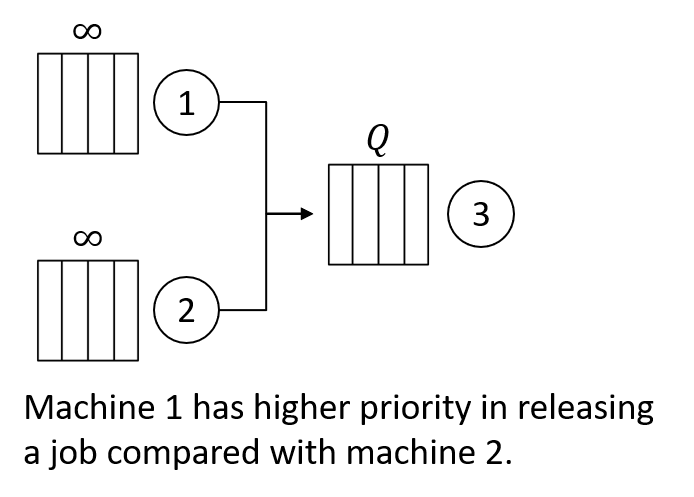
\includegraphics[width=0.9\textwidth]{Figures/merge.png}
	\caption{Example: merge.}
\end{figure}

\begin{table}[h]
	\begin{tabular}{|llllll|}\hline
		Variable&Event & Condition to schedule & Delay&\# executions& State change\\\hline
		$e^{s,1}$&Start m1 	& $m^1\le 0$ & $0$&1& $m^1++$ \\\hline
		$e^{f,1}$&Finish m1 & $1\le m^1\le 1$ 	& $t^1$ &1& $m^1++$\\\hline
		$e^{d,1}$&Depart m1& $m^1\ge2\ AND$&$0$ &1 & $m^1 = m^1-2,\ q--$\\
											&&$ q\ge 1$ &&&\\\hline
		$e^{s,2}$&Start m2 	& $m^2\le 0$ & $0$ &1& $m^2++$ \\	\hline
		$e^{f,2}$&Finish m2 & $1\le m^2\le 1$ 	& $t^2$ &1 & $m^2++$\\\hline
		$e^{d,2}$&Depart m2& $m^2\ge2\ AND$&$0$  &1& $m^2=m^2-2,\ q--$\\
						&&$\ q\ge 1\ AND$&&&\\
						&&$\ m^1\le 1 $ & &&\\\hline
		$e^{s,3}$& Start m3 & $m^3 \le 0\ AND$&$0$  &1& $m^3++,\ q++$\\
						&&$\ q\le Q-1$ & &&\\\hline
		$e^{d,3}$& Depart m3 & $m^3 \ge 1$ & $t^3$  &1& $m^3--$\\\hline
	\end{tabular}
	\caption{Merge-S3M111}
\end{table}

MP model:
\begin{eqnarray}
\min{\sum_{k}\mathcal{E}_k}\\
e^{(\xi,j),1}_i - \mathcal{E}_{k}\ge M(w^{\xi,j}_{i,k}-1)&&\xi\in\{s,f,d\}, j\in\{1,2,3\},\forall i,k \\
\mathcal{E}_{k} - e^{(\xi,j),1}_i\ge M(w^{\xi,j}_{i,k}-1)&&\xi\in\{s,f,d\}, j\in\{1,2,3\},\forall i,k \\
\sum_{k} w^{\xi,j}_{i,k} =1&& \forall\ \xi\in\{s,f,d\}, j\in\{1,2,3\},i\\
\sum_{(\xi,j),i} w^{\xi,j}_{i,k} =1&& \forall\ k\\
\sum_{k} kw^{\xi,j}_{i+1,k} - \sum_{k} kw^{\xi,j}_{i,k} \ge 1&& \forall\  \xi\in\{s,f,d\}, j\in\{1,2,3\},i\\
e^{s,j,1}_{i} - e^{s,j,0}_{i} \ge 0 && j =1,2,3, \forall \ i\\
e^{f,j,1}_{i} - e^{f,j,0}_{i} \ge t^j_{i}&& j =1,2, \forall \ i\\
e^{d,j,1}_{i} - e^{d,j,0}_{i} \ge 0 && j =1,2, \forall \ i\\
e^{d,3,1}_{i} - e^{d,3,0}_{i} \ge t^3_{i}&&\forall \ i \\
e^{\xi,j,0}_i-\mathcal{E}_{k} \ge M(x^{\xi,j}_{i,k}-1)&& \forall\ \xi\in\{s,f,d\},j=1,2,3,k,i\\
\mathcal{E}_{k} -e^{\xi,j,0}_i\ge M(x^{\xi,j}_{i,k}-1)&& \forall\ \xi\in\{s,f,d\},j=1,2,3,k,i\\
m^j_k=m^j_{k-1} + \sum_{i=1}^{N^{j}} (w^{s,j}_{i,k}  + w^{f,j}_{i,k} - 2w^{d,j}_{i,k})&& j=1,2, \forall\ k\\
m^3_k=m^3_{k-1} + \sum_{i=1}^{N^{3}} (w^{s,3}_{i,k} - w^{d,3}_{i,k})&&\forall\ k\\
q_k = q_{k-1} + \sum_{i=1}^{N^{3}} w^{s,3}_{i,k} - \sum_{i=1}^{N^{1}} w^{d,1}_{i,k} - \sum_{i=1}^{N^{2}} w^{d,2}_{i,k}\\
m^j_k \ge M(z^{s,j}_{k}-1)&& j=1,2,3, \forall \ k\\
1- m^j_k \ge M(z^{f,j}_{k}-1)&& j=1,2, \forall \ k\\
m^j_k - 1 \ge M(z^{f,j}_{k}-1)&& j=1,2, \forall \ k\\
m^j_k - 2 \ge M(z^{d,j}_{k}-1)&& j=1,2, \forall \ k\\
q_k - 1 \ge M(z^{d,j}_{k}-1)&&  j=1,2, \forall \ k\\
1 - m^1_k \ge M(z^{d,2}_{k}-1)&& \forall\ k\\
m^3_k - 1 \ge M(z^{d,3}_{k}-1)&& \forall \ k\\
(Q-1) - q_k \ge M(z^{s,3}_{k}-1)&& \forall\ k\\
\sum_{k} x^{\xi,j}_{i,k} =1&& \forall\ \xi\in\{s,f,d\}, j=1,2,3, \forall\ i,k\\
\sum_{i=1}^{N^{j}}x^{\xi,j}_{i,k} \le z^{\xi,j}_{k}&& \forall\ \xi\in\{s,f,d\}, j=1,2,3, k\\
\sum_{k} kx^{\xi,j}_{i+1,k} - \sum_{k} kx^{\xi,j}_{i,k} \ge 0 && \forall\ \xi\in\{s,f,d\}, j=1,2,3, i
\end{eqnarray}

\newpage
\subsection{Merge - 2 machines in station 3}
\begin{table}[h]
	\begin{tabular}{|llll|}\hline
		Variable&Value & Initialization& Description\\\hline
		$e^1$& 0,1,2&  2 &number of empty machines in station 1 \\\hline
		$f^1$&0,1,2	& 0 & number of finished jobs in station 1\\\hline
		$e^2$&0,1&1&number of empty machines in station 2 \\\hline
		$f^2$&0,1&0&number of finished jobs in station 2 \\\hline
		$e^3$&0,1&1&number of empty machines in station 3  \\	\hline
		$q$& 0,...,Q&Q&  number of available spaces in queue\\\hline
	\end{tabular}
	\caption{State variables: Merge-S3M211}
\end{table}


\begin{table}[h]
	\begin{tabular}{|llllll|}\hline
		Variable&Event & Condition to schedule & Delay&\# executions& State change\\\hline
	ai 	$e^{f,1}$&Finish m1 &  $1 \le  e^1 \le 2$	& $t^1$ &2& $f^1++$\\\hline
		$e^{d,1}$&Depart m1& $1\le   f^1  \le 2\ AND$&$0$ &1 & $e^1++,\ f^1--,\ q--$\\
											&&$ 1\le q\le Q$ &&&\\\hline
		$e^{s,2}$&Start m2 	& $1\le e^2\le 1$ & $0$ &1& $e^2--$ \\	\hline
		$e^{f,2}$&Finish m2 & $1\le e^2\le 1$ 	& $t^2$ &1 & $f^2++$\\\hline
		$e^{d,2}$&Depart m2&$1\le f^2 \le 1\ AND$&$0$  &1& $f^2--,e^2++,\ q--$\\
		&&$\ 1\le q\le Q\ AND$&&&\\
		&&$\ 0\le f^1\le 0 $ & &&\\\hline
		$e^{s,3}$& Start m3 & $1\le e^3\le 1\ AND$&$0$  &1& $e^3--,\ q++$\\
		&&$\ 0\le q\le Q-1$ & &&\\\hline
		$e^{d,3}$& Depart m3 & $1 \le e^3\le 1\ AND $ & $t^3$  &1& $e^3++$\\\hline
		&&$\ 0\le q\le Q-1$ & &&\\\hline
	\end{tabular}
	\caption{Events: Merge-S3M211}
\end{table}



\newpage
\subsection{Failure}



\newpage
\subsection{Jobshop}


\subsection{Identifying Resource-type variables}


\section{Gradient-based approximate cut}
\subsection{Gradient estimation}
\subsection{Gradient-based feasibility cut}


\section{Combinatorial cut generation}
\subsection{Combinatorial cut}
\subsection{Heuristic for tightening Exact combinatorial cut}

\section{Feasibility-cut-based algorithm}
The complete algorithm for solving RAP--PC is summarized in Algorithm 1. The resource capacities are initialized to the lower bound. The searching region of RAP--PC--MIP is initialized to $\Bbb{X}$, and the lower and upper bounds of the objective function, $C^L$ and $C^U$, respectively,  are set considering the upper bound and lower bound of the capacity of each resource. Lines 7 to 11 show that approximate cuts are generated and used in the model when infeasible solutions are found. Once a feasible solution is found, the upper bound $C^U$, which is also the incumbent solution, can be updated after comparing the value of the found feasible solution and that of the current incumbent. Then, all the currently used approximate cuts are replaced by exact cuts of the DIS. If there are only exact cuts in RAP--PC--MIP, the solution is the new lower bound $C^L$. The algorithm terminates when the gap between the upper bound and lower bound is within a tolerance or the time limit is exceeded.

\begin{algorithm}[h]
	\label{algo:}
	\caption{MIP--based algorithm.}
	\begin{algorithmic}[1]
		\REQUIRE ~~\\
		Lower bound $\mathbf{a}=[a_1,...,a_J]$ and upper bound $\mathbf{b}=[b_1,...,b_J]$ of resource capacity $\mathbf{x}$, such that $a_j\le x_j\le b_j\ \forall\ j=1,...,J$. \\
		Tolerance of optimality gap $\varepsilon_{opt}$.\\
		Optional input: time limit of the algorithm $T_{lim}$.\\
		\ENSURE ~~\\
		Sample-path global optimal $\mathbf{x}^*$.\\
		\STATE Initialize system with lower bound $\mathbf{x}\leftarrow\mathbf{a}$
		\STATE Initialize incumbent with upper bound $\mathbf{x}^*\leftarrow\mathbf{b}$. 
		\STATE Initialize lower bound of the objective $C^{L}\leftarrow\mathbf{c}^T\mathbf{a}$.
		\STATE Initialize upper bound of the objective $C^{U}\leftarrow\mathbf{c}^T\mathbf{b}$.
		\STATE Add initial constraints which defines $\Bbb{X}$ to the RAP--PC--MIP.
		\WHILE {$C^{U}-C^{L}>\varepsilon_{opt}$ and $T_{lim}$ is not exceeded.}
		\WHILE {There exists at least one violated performance constraint}
		\STATE Generate one approximate cut $CA(\bar{\mathbf{x}},l)$ for each violated constraints $l$ and add all the generated cuts to the RAP--PC--MIP.
		\STATE $\bar{\mathbf{x}}\leftarrow$ solution of the RAP--PC--MIP.
		\STATE Simulate the system of $\bar{\mathbf{x}}$.
		\ENDWHILE
		\STATE Update upper bound and incumbent $C^{U}\leftarrow\mathbf{c}^T\bar{\mathbf{x}},\ \mathbf{x}^*\leftarrow \bar{\mathbf{x}}$ if $\mathbf{c}^T\bar{\mathbf{x}}< C^{U}$.
		\IF {There exist approximate cuts in RAP--PC--MIP}
		\STATE For all the currently used approximate cuts $CA(\bar{\mathbf{x}}^r,l)$, find dominating infeasible solution $\bar{\mathbf{x}}_d(\bar{\mathbf{x}}^r)$ and replace approximate cuts $CA(\bar{\mathbf{x}}^r,l)$ by exact cuts $CE(\bar{\mathbf{x}}_d(\bar{\mathbf{x}}^r),l)$ of the DIS.
		\STATE $\bar{\mathbf{x}}\leftarrow$ solution of the RAP--PC--MIP.
		\STATE Simulate the system of $\bar{\mathbf{x}}$.
		\STATE Update lower bound $C^L\leftarrow \max\{\mathbf{c}^T\bar{\mathbf{x}},\ C^L\}$.
		\ENDIF	
		\ENDWHILE
	\end{algorithmic}
\end{algorithm}


\section{Numerical analysis}
\subsection{Multiple-server merge}
A multiple-server merge queueing system is shown in Figure \ref{fig:multimerge}. The multiple-server merge queue is a generalization of the system presented in Section 4.1, where the number of parallel servers in station 1, 2 and 3 is equal to $s^1$, $s^2$ and $s^3$, respectively. The state variables are changed accordingly. To describe the state of multiple-server station $j$, two state variables $g^{j}$ and $h^{j}$ are needed to represent the number of idle servers and the number of finished jobs of each the station. The state variable $q$ is used to represent the number of available space in buffer 3. 

\begin{figure}[h]
	\centering
	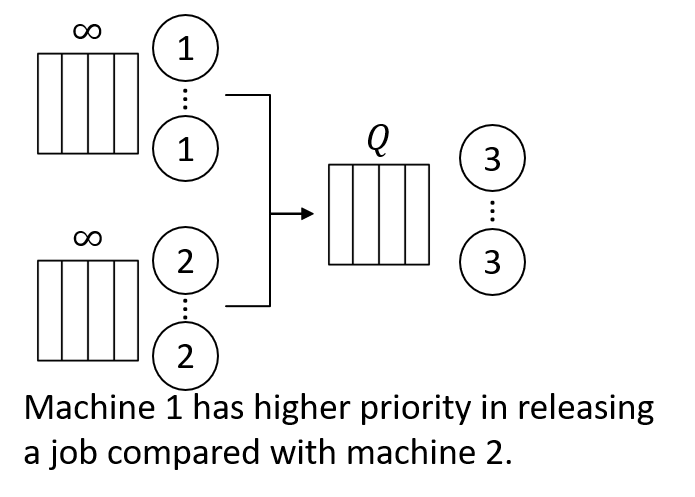
\includegraphics[width=0.4\textwidth]{Figures/multimerge.png}
	\caption{Example: multi-server merge.}
	\label{fig:multimerge}
\end{figure}


The events composing the DES model are shown in Table \ref{tab:multimerge}. The start event of station 1 and 2 is scheduled when there are at least one empty server, and their execution decreases the number of empty servers by one. The scheduling condition of finish event $e^{f,j}$ is the same as $e^{s,j}$, but its execution will increase the number of finished jobs by one. Event $e^{f,j}$ is a multi-execution event with positive delays, an event to count the number of executions of it should be introduced. However, the event $e^{s,j}$ plays that role and the number of executions in the event list is equal to $(s^j-g^j)$. Similarly with single-server system, the departure of station 1 requires that there is at least one finished job in the station and there is at least one space available in buffer 3, but the departure of station 2 also requires that there is no finished job in station 1. The departure of station 1 and 2 will increase the number of empty servers by one, decrease the number of finished jobs by one and decrease the number of available space by one. As for station 3, the start and departure event can be scheduled if there is at least one empty server and one job in buffer 3. Thus, $e^{s,3}$ is used to count the number executions in the event list of $e^{d,3}$. Execution of $e^{s,3}$ will decrease the number of empty server by one and increase the available space in buffer 3 by one.

\begin{table}[h]
	\begin{tabular}{|llllll|}\hline
		Variable&Event & Condition to schedule & Delay&$\beta^{\xi}$& State change\\\hline
		$e^{s,1}$&Start 1 	& $1\le g^1$ & $0$&1& $g^1--$ \\\hline
		$e^{f,1}$&Finish 1 & $1\le g^1$ 	& $t^1$ &$s^1$& $h^1++$\\\hline 
		$e^{d,1}$&Depart 1& $1\le h^1 \&\  q\ge 1$&$0$ &1 & $g^1++,h^1--,\ q--$\\\hline
		$e^{s,2}$&Start 2 	& $1\le g^2$ & $0$ &1& $g^2--$ \\	\hline
		$e^{f,2}$&Finish 2 & $1\le g^2$ 	& $t^2$ &$s^2$ & $h^2++$\\\hline
		$e^{d,2}$&Depart 2& $1\le h^2\ \&\ q\ge 1\ \&$&$0$  &1&  $g^2++,h^2--,\ q--$\\
		&&$\ h^1\le 0 $ & &&\\\hline
		$e^{s,3}$& Start 3 & $1\le g^3\ \&\ q\le Q-1$&$0$  &1& $g^3--,\ q++$\\\hline
		$e^{d,3}$& Depart 3 & $1\le g^3\ \&\ q\le Q-1$ & $t^3$  &$s^3$& $g^3++$\\\hline
	\end{tabular}
	\caption{Events to simulate a multi-server merge queueing system.}
	\label{tab:multimerge}
\end{table}

\section{Conclusion}




%Reference
\bibliographystyle{apacite}
\bibliography{RAP}

\end{document}
